\chapter{Mixed-Integer Linear Modelling and Analysis of Historical Schedules}
\label{chapter: 2-Evaluating Royal Mail Historical Data}

%%%%%%%%%%%%%%%%%%%%%%%%%%%%%%%%%%%%%%%%%%%%%%%%%%%%%%%%%%%%%%%%%%%%%%%%%%%%%%% SECTION %%%%%%%%%%%%%%%%%%%%%%%%%%%%%%%%%%%%%%%%%%%%%%%%%%%%%%%%%%%%%%%%%%%%%%%%%%%%%%
This chapter concerns the formulation of an initial set of models used to provide a first assessment on the opportunity for optimisation that is available in our problem. The goal of this analysis is to corroborate the quest of this dissertation to investigate the opportunity for efficiency gains and optimisation of the current practices run by Royal Mail. 

\vspace{\baselineskip}
\noindent
Section \ref{section: 4.1} starts by defining the playing field within which our models will be developed. It also provides an overview of the actual historical practices implemented by Royal Mail building upon the high-level overview seen in Chapter \ref{chapter: Problem Definition}. Sections \ref{section:Makespan Scheduling-content}-\ref{section: Pre-emptive} each involve the study of a different model, and they all follow a similar organisation. They begin by outlining the motivation behind the use of each of the models, and the goal we wish to achieve with each one. They then present the first set of results of this dissertation, outlining the efficiency gains that can be made for the instances of the supplied dataset.
%%%%%%%%%%%%%%%%%%%%%%%%%%%%%%%%%%%%%%%%%%%%%%%%%%%%%%%%%%%%%%%%%%%%%%%%%%%%%%% SECTION %%%%%%%%%%%%%%%%%%%%%%%%%%%%%%%%%%%%%%%%%%%%%%%%%%%%%%%%%%%%%%%%%%%%%%%%%%%%%%

\section{Modelling Environment}
\label{section: 4.1}
To develop this first set of model formulations, we assume that the schedule instances contain \textbf{fixed duties} with a concrete \texttt{start\_time}, and \texttt{end\_time}. Multiple duties are being run in parallel each day. Our goal is to allocate the trips (i.e. atomic blocks) efficiently to those available duties. We assume carte blanche in regards to our flexibility in allocating a block to a duty by neglecting any restrictions as to whether or not we can move a block. We also render our data points agnostic to any semantics associated with each trip\footnote{e.g. the distance between locations or the day on which each shift should occurs} and assume that all blocks are equivalent in their significance, and are merely characterised by their parameters. These abstractions will enable us to determine the maximum room for improvement that exists in efficiently allocating blocks to each duty establishing an upper bound in regards to the degree to which we can aim to optimise.

%%%%%%%%%%%%%%%%%%%%%%%%%%%%%%%%%%%%%%%%%%%%%%%%%%%%%%%%%%%%%%%%%%%%%%%%%%%%%%% sub-SECTION %%%%%%%%%%%%%%%%%%%%%%%%%%%%%%%%%%%%%%%%%%%%%%%%%%%%%%%%%%%%%%%%%%%%%%%%%%%%%%
\vspace{\baselineskip}
\noindent
The set of assumptions mentioned are succinctly summarised below:


%%%%%%%%%%%%%%%%%%%%%%%%%%%%%%%%%%%%%%%%%%%%%%%%%%%%%%%%%%%%%%%%%%%%%%%%%%%%%%% Table %%%%%%%%%%%%%%%%%%%%%%%%%%%%%%%%%%%%%%%%%%%%%%%%%%%%%%%%%%%%%%%%%%%%%%%%%%%%%%

	\begin{table}[ht]
	\renewcommand{\arraystretch}{1.7} %adds space between cells of a table
		\centering
		\begin{tabular}{|c |p{0.9\textwidth}|} 
			\multicolumn{2}{c}{\textbf{Simplifying Assumptions}} \\
		    \hline
			\textbf{(1)}  & The \textbf{duration} of a \textbf{block} stays \textbf{constant}, irrespective of the timing of its occurrence.\\
            \hline
            \textbf{(2)}  & The \texttt{start}, \texttt{end} times and \textbf{durations} of duties remain fixed. \\
            \hline
            \textbf{(3)}  &\textbf{Atomic blocks} are \textbf{freely interchangeable}, within the spectrum of a schedule.\\
			\hline
			\textbf{(4)}  & The \textbf{routes} are \textbf{fixed}, and we \textbf{maintain} the \textbf{order} with which we visit external locations.\\
			\hline
		\end{tabular} 
	\end{table}
	
\vspace{\baselineskip}
\noindent
The first two assumptions, capture the fact that our proposed schedules respect the principle of \textbf{conservation of time}. Our models receive as input an instance that contains blocks inside duties the sum of the durations of which gives us the \texttt{overall labor time} to be scheduled. The schedules that are generated from our algorithms have the same blocks, covering the same \texttt{overall labor time} with the only difference being the \textbf{arrangement}, of those blocks in the duties. The third assumptions, refers to our \textit{assignment policy} of blocks to duties, and the fact that it is completely open-ended giving the schedule total freedom over which duty, and at what point in time to assign a block. Finally, the last assumption reiterates that we do not focus on the routing aspect of this Vehicle-Routing like problem but only study its scheduling portion.
	

	
	%%%%%%%%%%%%%%%%%%%%%%%%%%%%%%%%%%%%%%%%%%%%%%%%%%%%%%%%%%%%%%%%%%%%%%%%%%%%%%% sub-SECTION %%%%%%%%%%%%%%%%%%%%%%%%%%%%%%%%%%%%%%%%%%%%%%%%%%%%%%%%%%%%%%%%%%%%%%%%%%%%%%
	
\subsection*{Evaluation of Historical Schedules}
To begin assessing the performance of our optimised schedule we must first look at the schedules currently run by Royal Mail which we refer to as the \textbf{historical} instance.

%%%%%%%%%%%%%%%%%%%%%%%%%%%%%%%%%%%%%%%%%%%%%%%%%%%%%%%%%%%%%%%%%%%%%% Table %%%%%%%%%%%%%%%%%%%%%%%%%%%%%%%%%%%%%%%%%%%%%%%

\begin{table}[h]
\small
    \centering 
    \begin{tabular}{|c|c|c|c|c|c|c|}
        \hline
        \textbf{Instance} & \multicolumn{3}{|c|}{ \textbf{Characteristics}} & \multicolumn{3}{|c|}{ \textbf{Blocks (HH:mm)}}  \\
        \hline
        & \texttt{Duties} & \texttt{Blocks} & \texttt{Activities} & \texttt{Average} &  \texttt{Minimum} & \texttt{Maximum} \\
        \hline
        Historical & 183 & 462 & 3,285 & 03:05 & 00:40 & 08:25 \\
        \hline
    \end{tabular}%
    \medbreak
\end{table}


\vspace{\baselineskip}
\noindent
The historical schedules which our model is given as an input are driven by an instance $I = \langle{m},B\rangle{}$ of the problem where 462 blocks are allocated among a set of 183 duties over the period of a week\footnote{As input we provide the Finalised Dataset (Cleaned) from Section \ref{section: Data Cleaning} of the previous chapter that we henceforth refer to as the Historical Schedule.}. The minimal processing time $p_{j}$ was that of a round-trip lasting only 40 minutes while the longest trips lasted up to 8 hours and 25 minutes. On average a round-trip is expected to last 3 hours and 5 minutes among the historical schedules. 


%%%%%%%%%%%%%%%%%%%%%%%%%%%%%%%%%%%%%%%%%%%%%%%%%%%%%%%%%%%%%%%%%%%%%% Table %%%%%%%%%%%%%%%%%%%%%%%%%%%%%%%%%%%%%%%%%%%%%%%

\begin{table}[h]
\small
    \centering 
    \begin{tabular}{|c|c|c|c|c|}
        \hline
        \textbf{Schedule} & \multicolumn{3}{|c|}{ \textbf{Duties (HH:mm)}} & \textbf{Total Time (HH:mm)}  \\
        \hline
        & \texttt{Average} &  \texttt{Minimum} & \texttt{Makespan} & \\
        \hline
        Historical & 07:50 & 02:50 & 11:50 & 1,435:22 \\
        \hline
    \end{tabular}%
    \medbreak
\end{table}
\vspace{\baselineskip}
\noindent
We proceeded to plot a histogram of the duty structure of the historical schedule, seen in Figure \ref{fig: Historical for Evaluation.}. In that diagram we have fitted the historical workload into class intervals or histogram bins that represent durations of duties according to the duties of the historical schedule. The purpose of this figure is to show us how much each driver works historically. Indeed, there is a \textbf{noticeable variation}. We see some drivers work for around 2 hours whereas others for close to 12 hours and in general there are some \textbf{significant fluctuations}, which provokes a waste of labour hours. In general, there are people asked to perform duties in excess of 9 hours, hence requiring \textbf{overtimes}, which might prove costly for the company. Hence, envisioning a more balanced schedule we wanted to see if it is possible to have a solution that balances the workload more uniformly. This motivated the experiment run in Section \ref{section:Makespan Scheduling-content}, where since our goal is a balanced schedule we choose a formulation based on the \textit{Makespan Scheduling} model first seen in Section \ref{section:Makespan Scheduling}. The motivation behind this choice is that as was explained in Section \ref{section:Makespan Scheduling}, a schedule with a minimised \textit{makespan} usually achieves a \textbf{well-balanced} sequence of the tasks processed \cite{DUMMY:2}.


%%%%%%%%%%%%%%%%%%%%%%%%%%%%%%%%%%%%%%%%%%%%%%%%%%%%%%%%%%%%%%%%%%%%%%%%%%%%% Figure %%%%%%%%%%%%%%%%%%%%%%%%%%%%%%%%%%%%%%%%%%%%%%%%%%%%%%%%%%%%%%%%%%%%%%%%%%%%%%

\begin{figure}[ht]
\begin{center}
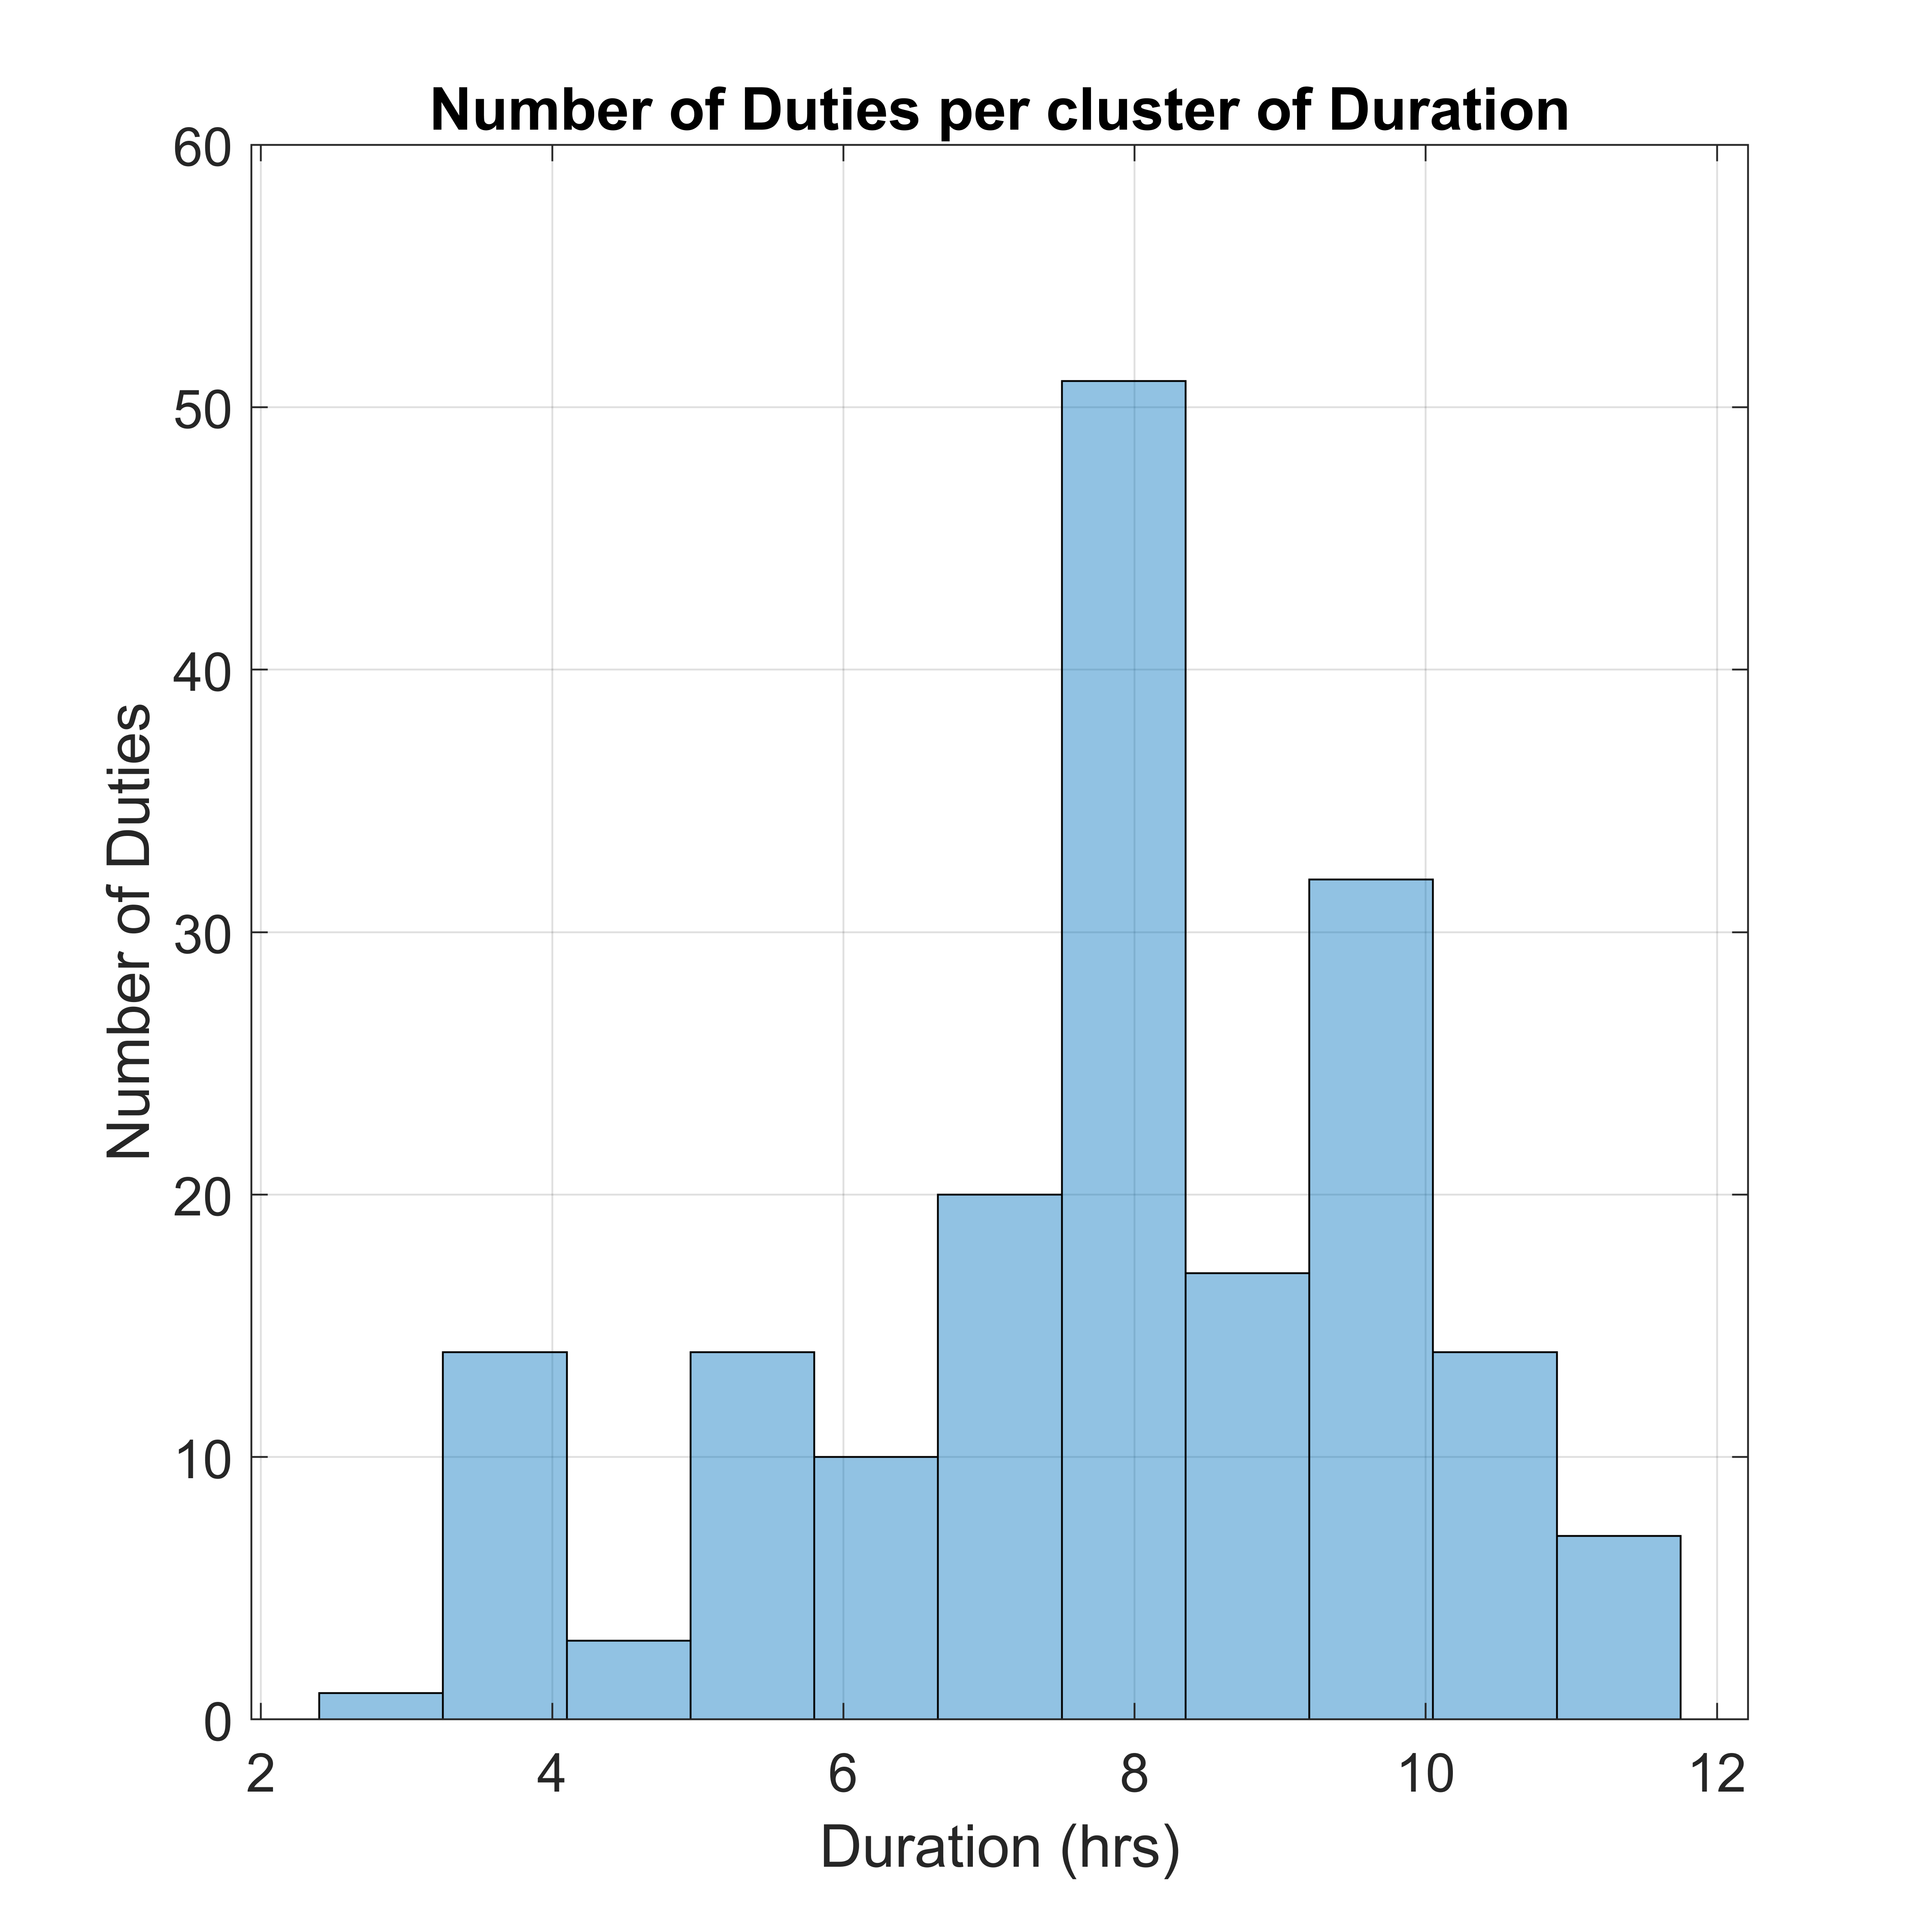
\includegraphics[width=0.46\linewidth]{[1] - chapter/Image Files/Historical-for-evaluation.png}
    
\end{center}
   \caption{The histogram provides an overview of the overall $Duty$ lengths featured in the \textbf{Historical Schedule}.}
\label{fig: Historical for Evaluation.}
\end{figure}

%%%%%%%%%%%%%%%%%%%%%%%%%%%%%%%%%%%%%%%%%%%%%%%%%%%%%%%%%%%%%%%%%%%%%%%%%%%%%%% SUBSECTION %%%%%%%%%%%%%%%%%%%%%%%%%%%%%%%%%%%%%%%%%%%%%%%%%%%%%%%%%%%%%%%%%%%%%%%%%%%%%%

\section{Load Balancing}
\label{section:Makespan Scheduling-content}
With the goal of finding a more balanced schedule in terms of duty length the \textit{Makespan Scheduling} formulation attempts to minimise the overall duration of the schedule, the \textbf{makespan}. The goal is for the resulting optimised schedule to decrease the amount of time for which a driver is generally occupied for, a practical advantage that we hope will be gained by a \textbf{balanced schedule}.

\vspace{\baselineskip}
\noindent
The two evaluation criteria that we need to examine to determine the success of our model are the degree to which the \textit{makespan is decreased} and a \textit{measure of uniformity} of the optimised schedule. Two ways to practically evaluate these two criteria is to look at the \textbf{(\%) makespan reduction} and the \textbf{(\%) standard deviation reduction ($\pmb{\sigma}$)} of the distribution of duties, respectively, compared to the instance that was provided as input to the model. Hence, for the experiments involving the Makespan model, we compare every schedule generated at each stage with respect to those two measures of success. 

\vspace{\baselineskip}
\noindent
An instance $I = \langle{m},B\rangle{}$ of the problem involves  an environment of $D=\{1,...,m\}$ parallel and identical duties, and a set of blocks $B =\{1,...,n\}$. Each duty may be assigned at most \textbf{one block per unit of time}, and once assigned a block it must execute it until its completion with no interruptions. In other words, this is a \textit{non-preemptive} model. %A duty is described by its start time $s_{i}$, and finish time $f_{i}$. The execution of any blocks for each duty must occur within the time horizon $f_{i}-s_{i}$. 
The blocks $j \in B$ are all associated with processing time $p_{j}$ as their one and only attribute. Mathematically the goal for this first stage of optimisation is to evenly allocate the blocks to each duty in a way that minimises the completion time of the last duty to be completed. 

\vspace{\baselineskip}
\noindent
The formulation utilised to perform this task is an adapted version %aka a variance
of the makespan scheduling model seen in Chapter \ref{chapter: Background}. We parallelise\footnote{The purpose of this parallelisation is to transform our problem into an equivalent problem to that studied in \cite{PRAKASH2010}, for which efficient algorithms for solving it have already been studied.} our problem with the problem observed in Section \ref{section:Makespan Scheduling}. We consider a \textbf{duty} as the \textit{machine} from formulation \ref{section:Makespan Scheduling} and a \textbf{block} as a \textit{job}, respectively. Hence, our formulation assigns blocks to duties. Binary variable $x_{i,j}$ dictates the assignment of a block $j$ to a duty $i$. The binary variable $x_{i,j}$ is equal to 1 if the atomic block $j \in B$ is assigned to duty $i \in D$, and 0 otherwise. Continuous variable $y$ contains the \textbf{makespan} of the schedule, which is what we are trying to minimise.  

%%%%%%%%%%%%%%%%%%%%%%%%%%%%%%%%%%%%%%%%%%%%%%%%%%%%%%%%%%%%%%%%%%%%%%%%%%%%%%% Maths %%%%%%%%%%%%%%%%%%%%%%%%%%%%%%%%%%%%%%%%%%%%%%%%%%%%%%%%%%%%%%%%%%%%%%%%%%%%%%

\vspace{\baselineskip}
\begin{equation}
\label{equation: Makespan Scheduling}
\begin{aligned}
&\text{minimise}
%& & y_{i}  \\ %\todo{why y and and not yi}
& & y  \\ 
& \text{subject to}
% & & y_{i} = \sum _{j=1}^n x_{i,j}p_{j}  \;\;\; &\forall \; i \in D\tag{1}\\   
& & y \geq \sum _{j=1}^n x_{i,j}p_{j}  \;\;\; &\forall \; i \in D\\   
& & &\sum _{i=1}^m x_{i,j} = 1 \;\;\; &\forall \; j \in B\\
% & & &\sum _{j=1}^n x_{i,j}p_{j} \leq f_{i}-s_{i} \;\;\; &\forall \; i \in D\\ %{\color{red} we deleted the constraint that involves the length of duty being less than end-start.}
& & & y\geq 0  \\
& & & x_{i,j} \in  \{ 0,1 \} \;\;\; &\forall \; j \in B, \; i \in D\\
\end{aligned}
\end{equation}

\vspace{\baselineskip}
\noindent
The objective is to get the \textbf{minimal} possible \textbf{makespan} that allows a feasible schedule. The first constraint assigns $y$ its definition of the \textbf{makespan} by making it equal to the completion time of the last atomic block to be executed. With the second constraint we make sure that each block is assigned to at least one but only one duty. The third and the fourth constraints enforce the continuous and integrality nature to the $y,x$ variables respectively, rendering this a \textit{MILP} problem.

%%%%%%%%%%%%%%%%%%%%%%%%%%%%%%%%%%%%%%%%%%%%%%%%%%%%%%%%%%%%%%%%%%%%%%%%%%%%%%% sub-SECTION %%%%%%%%%%%%%%%%%%%%%%%%%%%%%%%%%%%%%%%%%%%%%%%%%%%%%%%%%%%%%%%%%%%%%%%%%%%%%%

\subsection*{Evaluation}
In this initial model, we choose to focus on trying to shorten the \textbf{completion time} of the \textbf{longer lasting duty}, with the goal of obtaining \textbf{fairer shifts }that will have a more \textbf{uniform} allocation of the workload among drivers. In the historical schedule, the shortest shift lasts for 2 hours and 50 minutes while the longest one (i.e. the makespan) takes 11 hours and 50 minutes, as seen before. The historical allocation of blocks has been done heuristically, for the historical schedules, which is why cases of longer and shorter shifts than the average tend to occur. Taking as an example, the extremely short and long cases of shifts described above a closer observation shows that more than seven blocks (i.e. round-trips) were allocated to a driver as part of that longest shift, whereas just a single one was assigned to the shortest shift. Such observations motivate our efforts in striving to improve efficiency by minimising the duration of every duty to ensure a fairer allocation of the work load, since there seems to be a chance to remedy all these oddities of the historical schedule.

\vspace{\baselineskip}
\noindent
With regards to the objective of our model, the makespan, we need to be aware of a practical constraint that places a lower bound regarding the most minimum makespan that can be achieved in a feasible schedule. This constraint stems from the fact the there exist blocks of duration 8 hours and 25 minutes. According to assumption (4) of Section \ref{section: 4.1}, we cannot split a block into smaller sub-components so as to reduce its duration. Consequently, the \texttt{absolute theoretical limit} in regards to the most optimal schedule that we can hope to achieve will have a makespan equal to the duration of those maximum-lasting blocks. Such a schedule would contain duties that solely complete these 08:25 block and no other. Proposing a schedule with an 08:25 makespan or one close to it will constitute an efficient optimisation of the current practices. 

%%%%%%%%%%%%%%%%%%%%%%%%%%%%%%%%%%%%%%%%%%%%%%%%%%%%%%%%%%%%%%%%%%%%%%%%%%%%%%% Figure %%%%%%%%%%%%%%%%%%%%%%%%%%%%%%%%%%%%%%%%%%%%%%%%%%%%%%%%%%%%%%%%%%%%%%%%%%%%%%

\begin{figure}%
    \centering
    \subfloat[The duration of each duty before and after optimisation sorted in increasing duration.]{%\begin{center}
    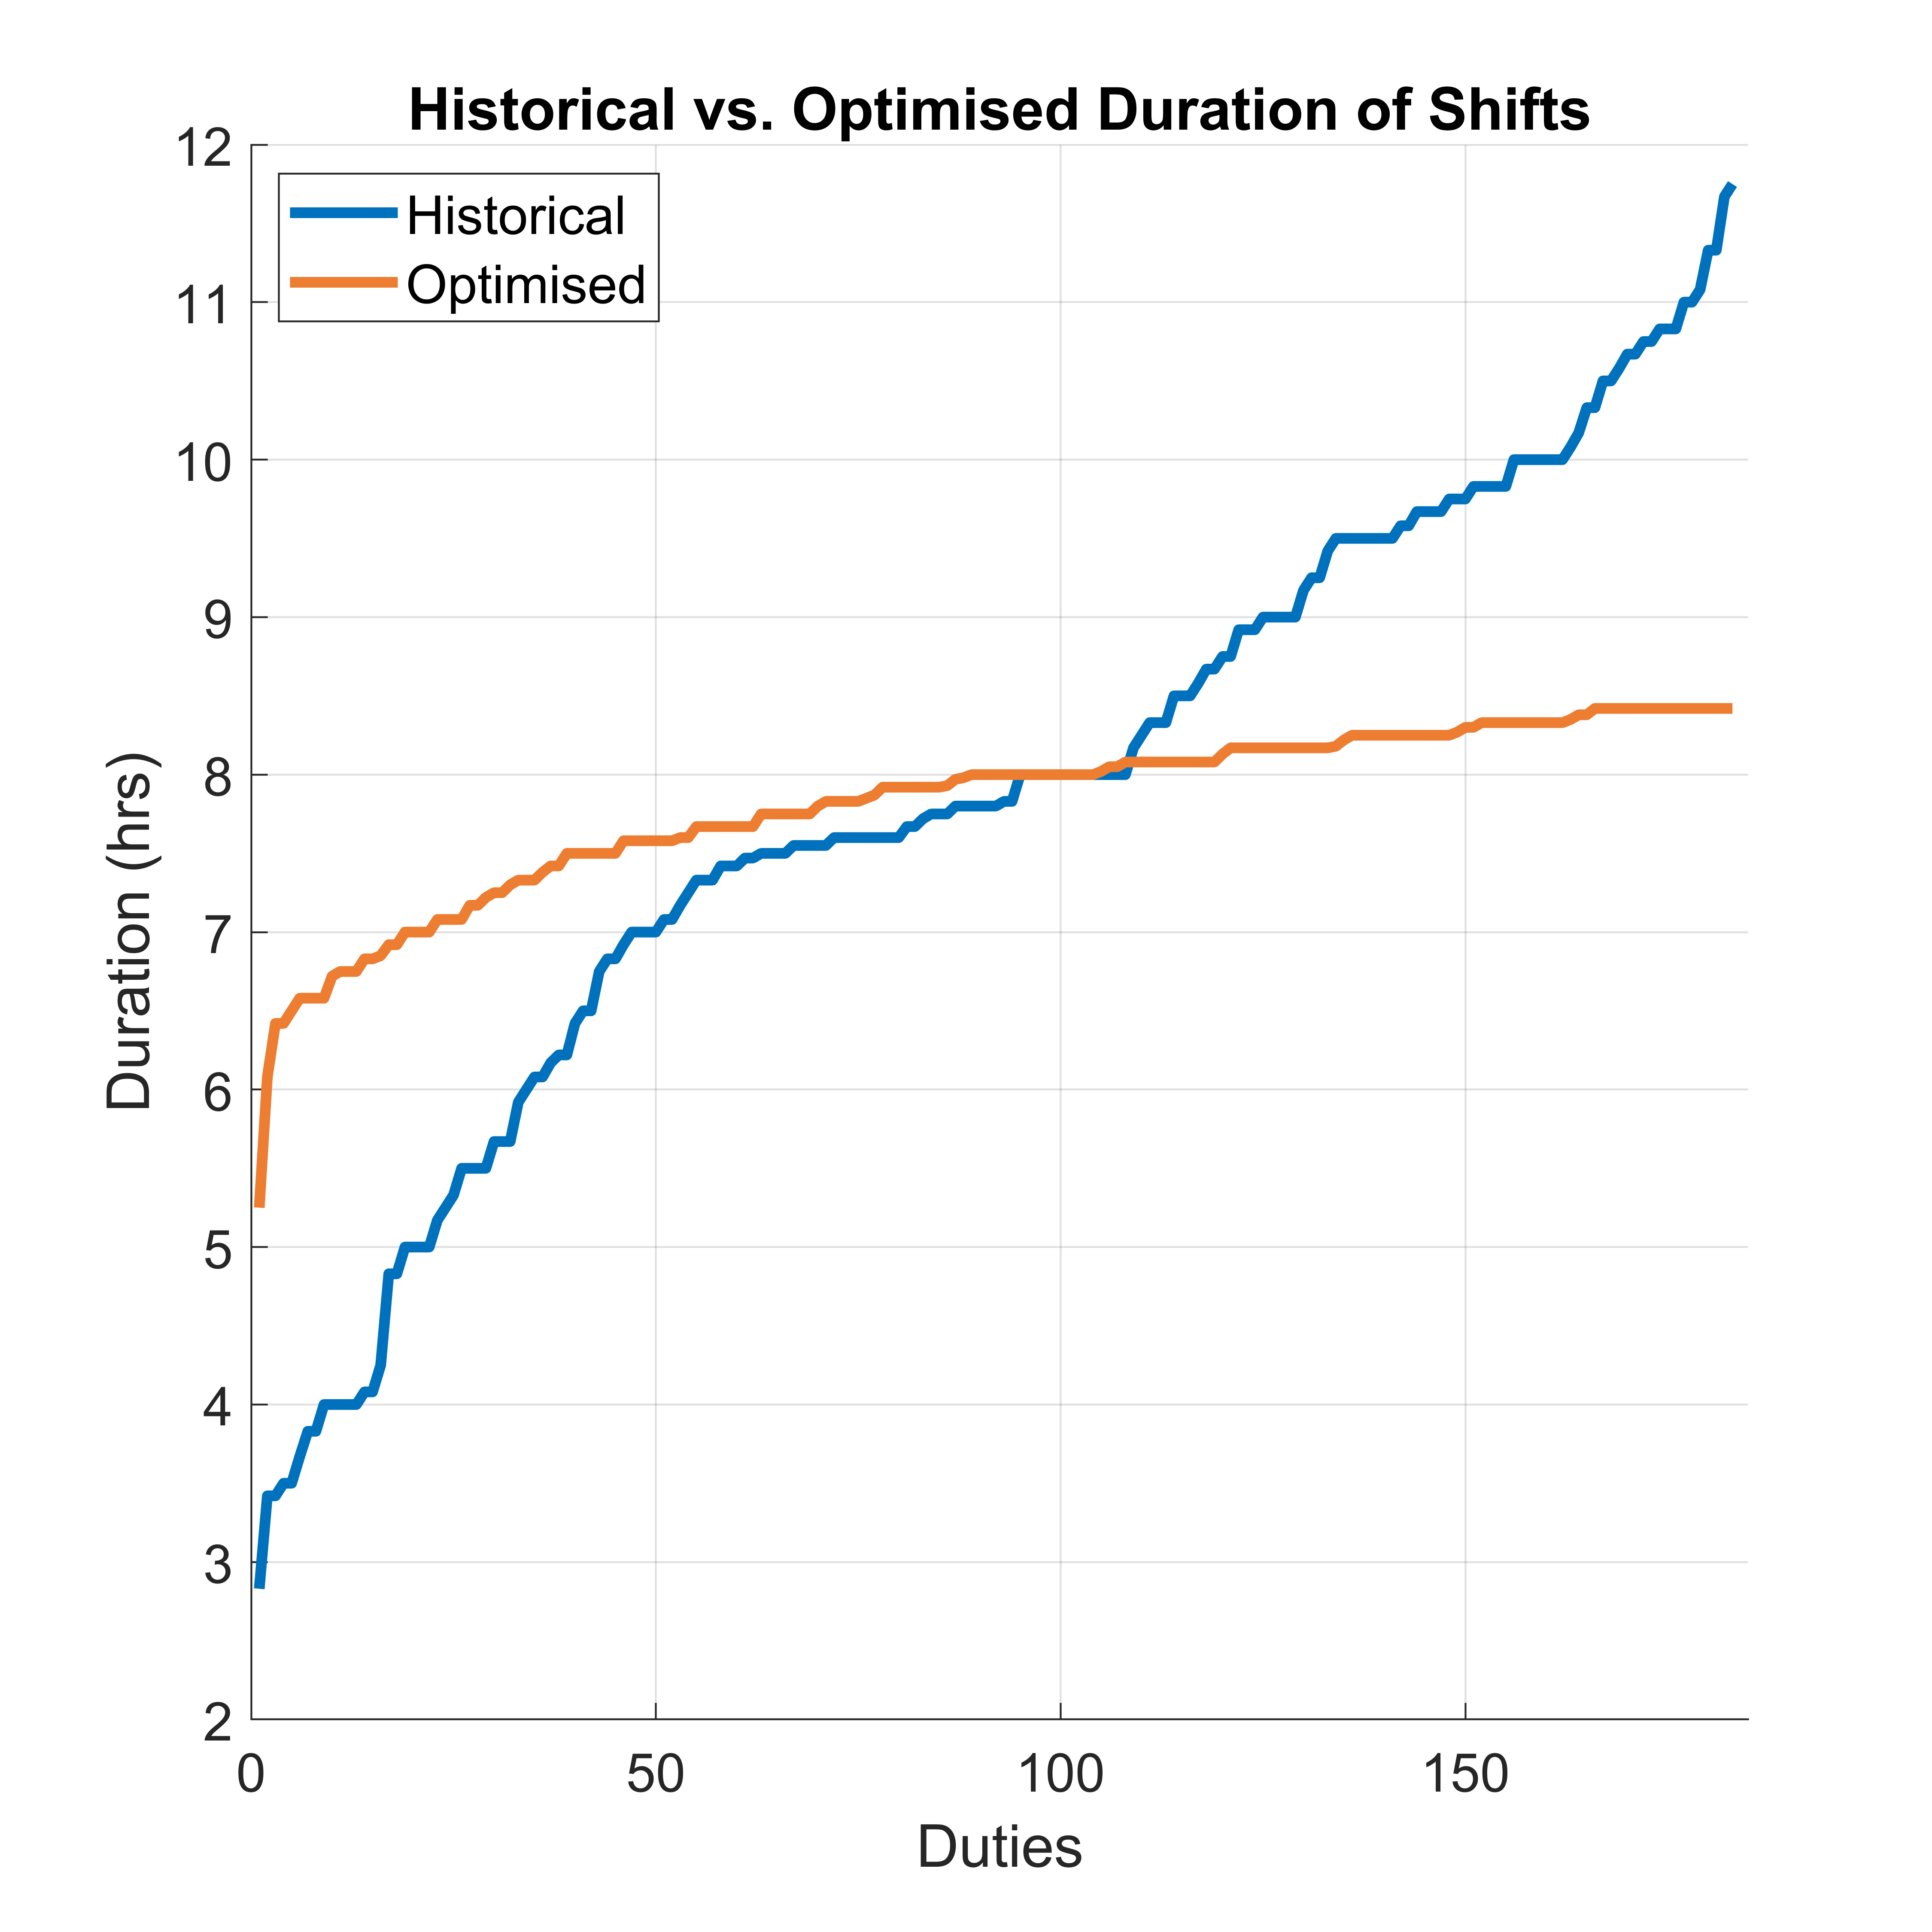
\includegraphics[width=0.46\linewidth]{[1] - chapter/Image Files/1-D1.png}
    }%\end{center}}%picture #1
    \qquad
    %picture #2
    \centering
    \subfloat[Histogram showing the improvement in the \textbf{uniformity} of duties.]{%\begin{center}
    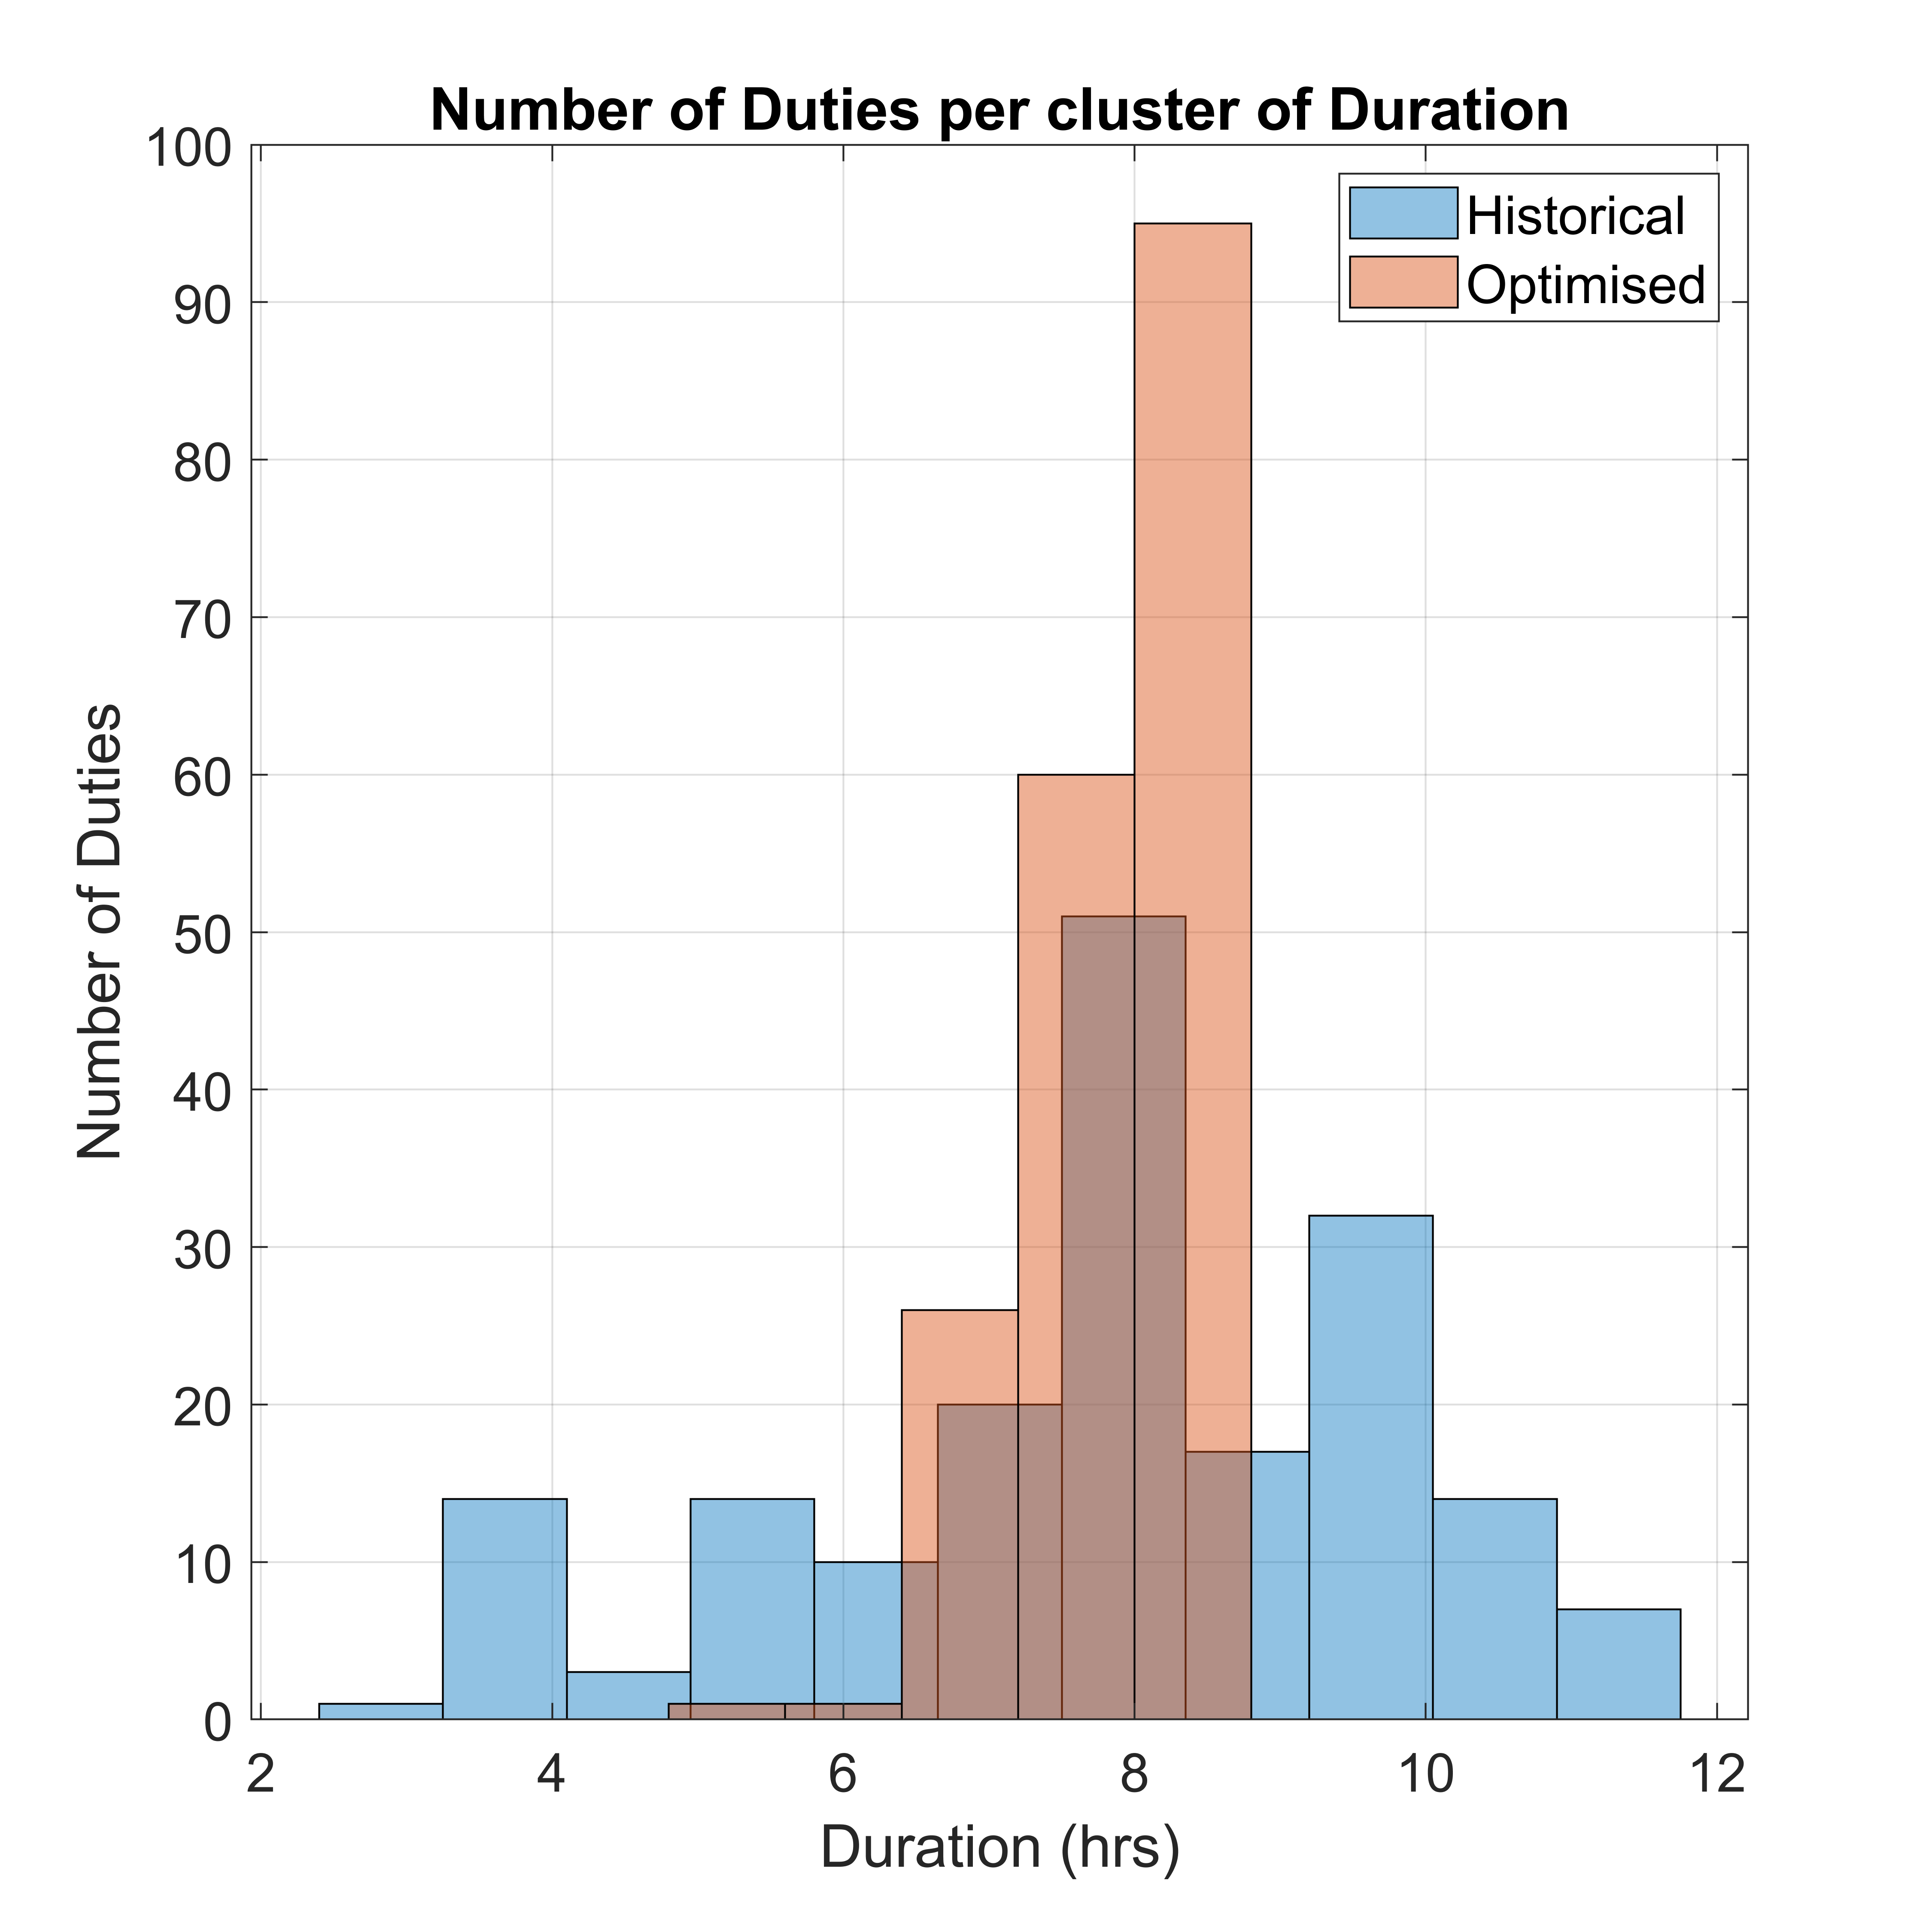
\includegraphics[width=0.46\linewidth]{[1] - chapter/Image Files/1-D1M1.png}
    }%\end{center}}%end of picture #2
    \caption{Figures illustrating the effects of the optimisation model on the historical duties.}%
    \label{fig:1-D1M1}%
\end{figure}

%%%%%%%%%%%%%%%%%%%%%%%%%%%%%%%%%%%%%%%%%%%%%%%%%%%%%%%%%%%%%%%%%%%%%%%%%%%%%%% sub-SECTION %%%%%%%%%%%%%%%%%%%%%%%%%%%%%%%%%%%%%%%%%%%%%%%%%%%%%%%%%%%%%%%%%%%%%%%%%%%%%%

\subsubsection*{Qualitative Results}
The application of the Makespan Scheduling model on the Historical dataset has the effect of \textit{flattening} the historical curve as seen in Figure \ref{fig:1-D1M1}(a), and hence concentrating the majority of the workload on duties that last as long as the makespan of the schedule, or less. 

\vspace{\baselineskip}
\noindent
The effect of our model is most noticeable in Figure \ref{fig:1-D1M1}(b) which plots the duration of each duty before and after the optimisation. We can observe how this first attempt at optimising the historical schedule results in a fairer distribution of labor time, since the majority of duties are now of similar length. There is also a big improvement in the \textbf{reduction of extremities} vis-\`a-vis extremely long and extremely short shifts, allowing us to prevent the occurrence of a large group of very long duties that are not efficient since they require drivers to complete overtimes. In a nutshell a reduction of the order of \textbf{72\%} in the \textbf{standard deviation ($\pmb{\sigma}$)} of the optimised schedule compared to the input instance encapsulates the fact that we have achieved our main goal of obtaining a more uniform schedule.

\subsubsection*{Numerical Results}

%%%%%%%%%%%%%%%%%%%%%%%%%%%%%%%%%%%%%%%%%%%%%%%%%%%%%%%%%%%%%%%%%%%%%% Table %%%%%%%%%%%%%%%%%%%%%%%%%%%%%%%%%%%%%%%%%%%%%%%

\begin{table}[h]
\small
    \centering 
    \begin{tabular}{|l|c|c|c|c|}
        \hline
        \textbf{Schedule} & \multicolumn{3}{|c|}{ \textbf{Duties (HH:mm)}} & \textbf{Total Time (HH:mm)}  \\
        \hline
        & \texttt{Average} &  \texttt{Minimum} & \texttt{Makespan} & \\
        \hline
        Historical & 07:50 & 02:50 & 11:50 & 1,435:22 \\
        \hline
        Historical\_Optimised & 07:50 & 05:15 & 08:25 & 1,435:22 \\
        \hline
    \end{tabular}%
    \medbreak
\end{table}


\vspace{\baselineskip}
\noindent
We have also achieved our main objective of minimising the \textit{maximum duty length} since the historical makespan was 11 hours and 45 minutes whereas in our revised schedule it is exactly 8 hours and 25 minutes hence, achieving the \texttt{absolute theoretical limit}. This accomplishment amounts to a \textbf{28\% reduction of the makespan} compared to the historical instance received as input. In essence, we have redistributed the load\footnote{The principle of \textbf{conservation of time} is respected as observed on the \texttt{Average} and Total Time columns of the table.} so that some people will not need to be working \textbf{overtimes} hence resulting in efficiency cost cuts for Royal Mail. A side-effect of our scheduling is that some drivers will be working a bit more. As far as Royal Mail is concerned this is a welcome change since it means we will be utilising the drivers' time better.

\vspace{\baselineskip}
\noindent
It is evident in the historical schedule in Figure \ref{fig:1-D1M1}(b) that duties lasting between 8-11.7 hours take a larger load of the work while the rest of the shifts carry out a smaller portion of the overall workload. By making an effort to redistribute the load in a more uniform fashion we are able to achieve a \textbf{fairer allocation} of the amount of work required by assigning the load of the long lasting shift to the frequently occurring shifts of up to 8 hours and 25 minutes. We distributed the load from the previously shorter and longer lasting shifts to those frequently occurring ones. The outcome, was an increase in the duration of the shorter lasting shifts resulting in a fairer allocation of the load. However, this also resulted in an increase in the frequency with which the around 8 hour lasting shifts occur. This is an unwanted side-effect of this redistribution of load since even though we reduce the toll taken by the most frequently occurring shift, we distribute a portion of it on the longer-lasting shifts which are already overwhelmed. 

\vspace{\baselineskip}
\noindent
A synopsis of the statistics that highlight the performance of our model for the Historical schedule as the input instance is found below:
%%%%%%%%%%%%%%%%%%%%%%%%%%%%%%%%%%%%%%%%%%%%%%%%%%%%%%%%%%%%%%%%%%%%%% Table %%%%%%%%%%%%%%%%%%%%%%%%%%%%%%%%%%%%%%%%%%%%%%%

\begin{table}[h]
\small
    \centering 
\begin{tabular}{c|c|c}
        \textbf{Schedule} & \textbf{Makespan Reduction (\%)} & Mean Deviation-\textbf{Reduction (\%)} \\
        \hline
         Historical\_Optimised & 28\% & 72\% \\
\end{tabular}
\end{table}

%%%%%%%%%%%%%%%%%%%%%%%%%%%%%%%%%%%%%%%%%%%%%%%%%%%%%%%%%%%%%%%%%%%%%%%%%%%%%%% sub-SECTION %%%%%%%%%%%%%%%%%%%%%%%%%%%%%%%%%%%%%%%%%%%%%%%%%%%%%%%%%%%%%%%%%%%%%%%%%%%%%%



%%%%%%%%%%%%%%%%%%%%%%%%%%%%%%%%%%%%%%%%%%%%%%%%%%%%%%%%%%%%%%%%%%%%%%%%%%%%%%% sub-SECTION %%%%%%%%%%%%%%%%%%%%%%%%%%%%%%%%%%%%%%%%%%%%%%%%%%%%%%%%%%%%%%%%%%%%%%%%%%%%%%

\subsection*{Evaluation - Optimising Redefined Instance}

%%%%%%%%%%%%%%%%%%%%%%%%%%%%%%%%%%%%%%%%%%%%%%%%%%%%%%%%%%%%%%%%%%%%%% Table %%%%%%%%%%%%%%%%%%%%%%%%%%%%%%%%%%%%%%%%%%%%%%%

\begin{table}[h]
\small
    \centering 
    \begin{tabular}{|c|c|c|c|c|c|c|}
        \hline
        \textbf{Instance} & \multicolumn{3}{|c|}{ \textbf{Characteristics}} & \multicolumn{3}{|c|}{ \textbf{Blocks (HH:mm)}}  \\
        \hline
        & \texttt{Duties} & \texttt{Blocks} & \texttt{Activities} & \texttt{Average} &  \texttt{Minimum} & \texttt{Maximum} \\
        \hline
        Historical & 183 & 462 & 3,285 & 03:05 & 00:40 & 08:25 \\
        \hline
        Redefined & 183 & 462 & 2,850 & 02:25 & 00:30 & 06:35 \\
        \hline
    \end{tabular}%
    \medbreak
\end{table}

\vspace{\baselineskip}
\noindent
We now apply model (\ref{equation: Makespan Scheduling}) to an instance of the Redefined\footnote{Introduced in Section \ref{section: Redefined Dataset} of the previous chapter.} blocks and compare the model's performance with the optimal schedule, previously generated. As mentioned in Section \ref{section: Redefined Dataset}, the Redefined instance is expected to lead us to a better solution, with respect to makespan, since it contains \textbf{less activities} and consequently \textbf{less labour hours to be scheduled}, due the deletion of the non-useful activities. 

%%%%%%%%%%%%%%%%%%%%%%%%%%%%%%%%%%%%%%%%%%%%%%%%%%%%%%%%%%%%%%%%%%%%%%%%%%%%%%% Figure %%%%%%%%%%%%%%%%%%%%%%%%%%%%%%%%%%%%%%%%%%%%%%%%%%%%%%%%%%%%%%%%%%%%%%%%%%%%%%

\begin{figure}%
    \centering
    \subfloat[The duration of each duty before and after optimisation sorted in increasing duration.]{%\begin{center}
    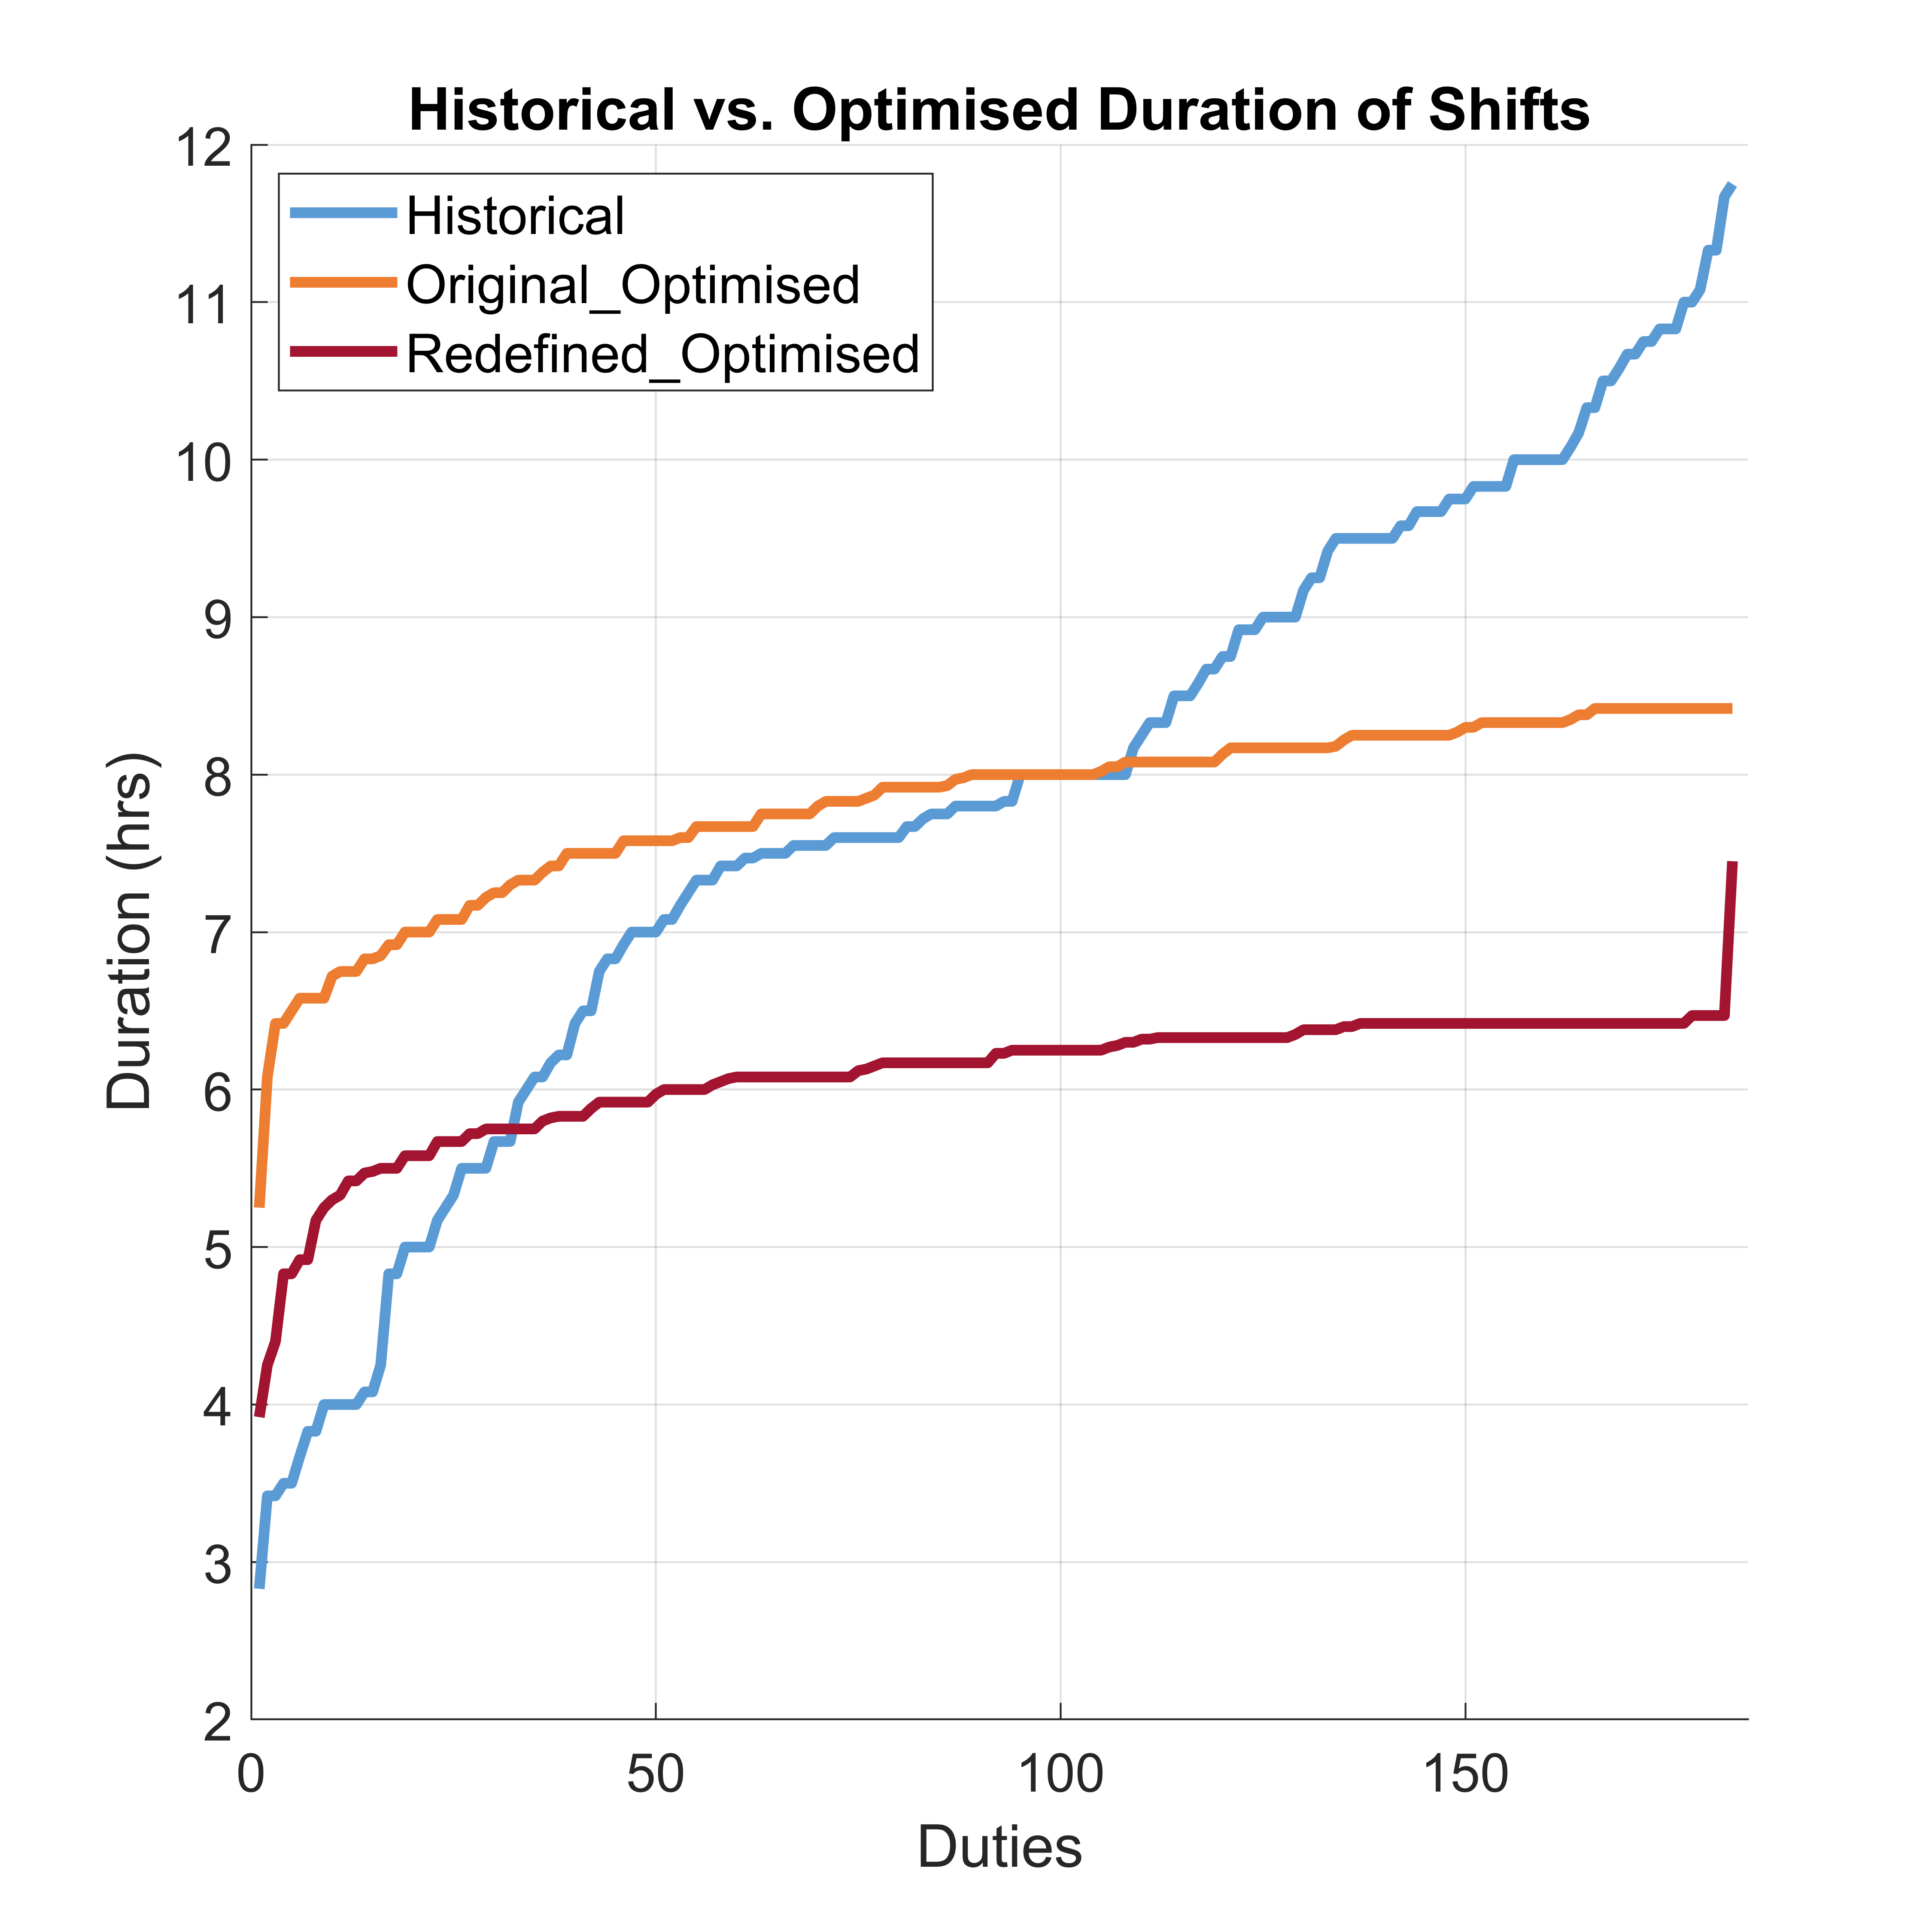
\includegraphics[width=0.46\linewidth]{[1] - chapter/Image Files/1-D2.png}
    }%\end{center}}%picture #1
    \qquad
    %picture #2
    \centering
    \subfloat[Histogram showing the improvement in the uniformity of duties.]{%\begin{center}
    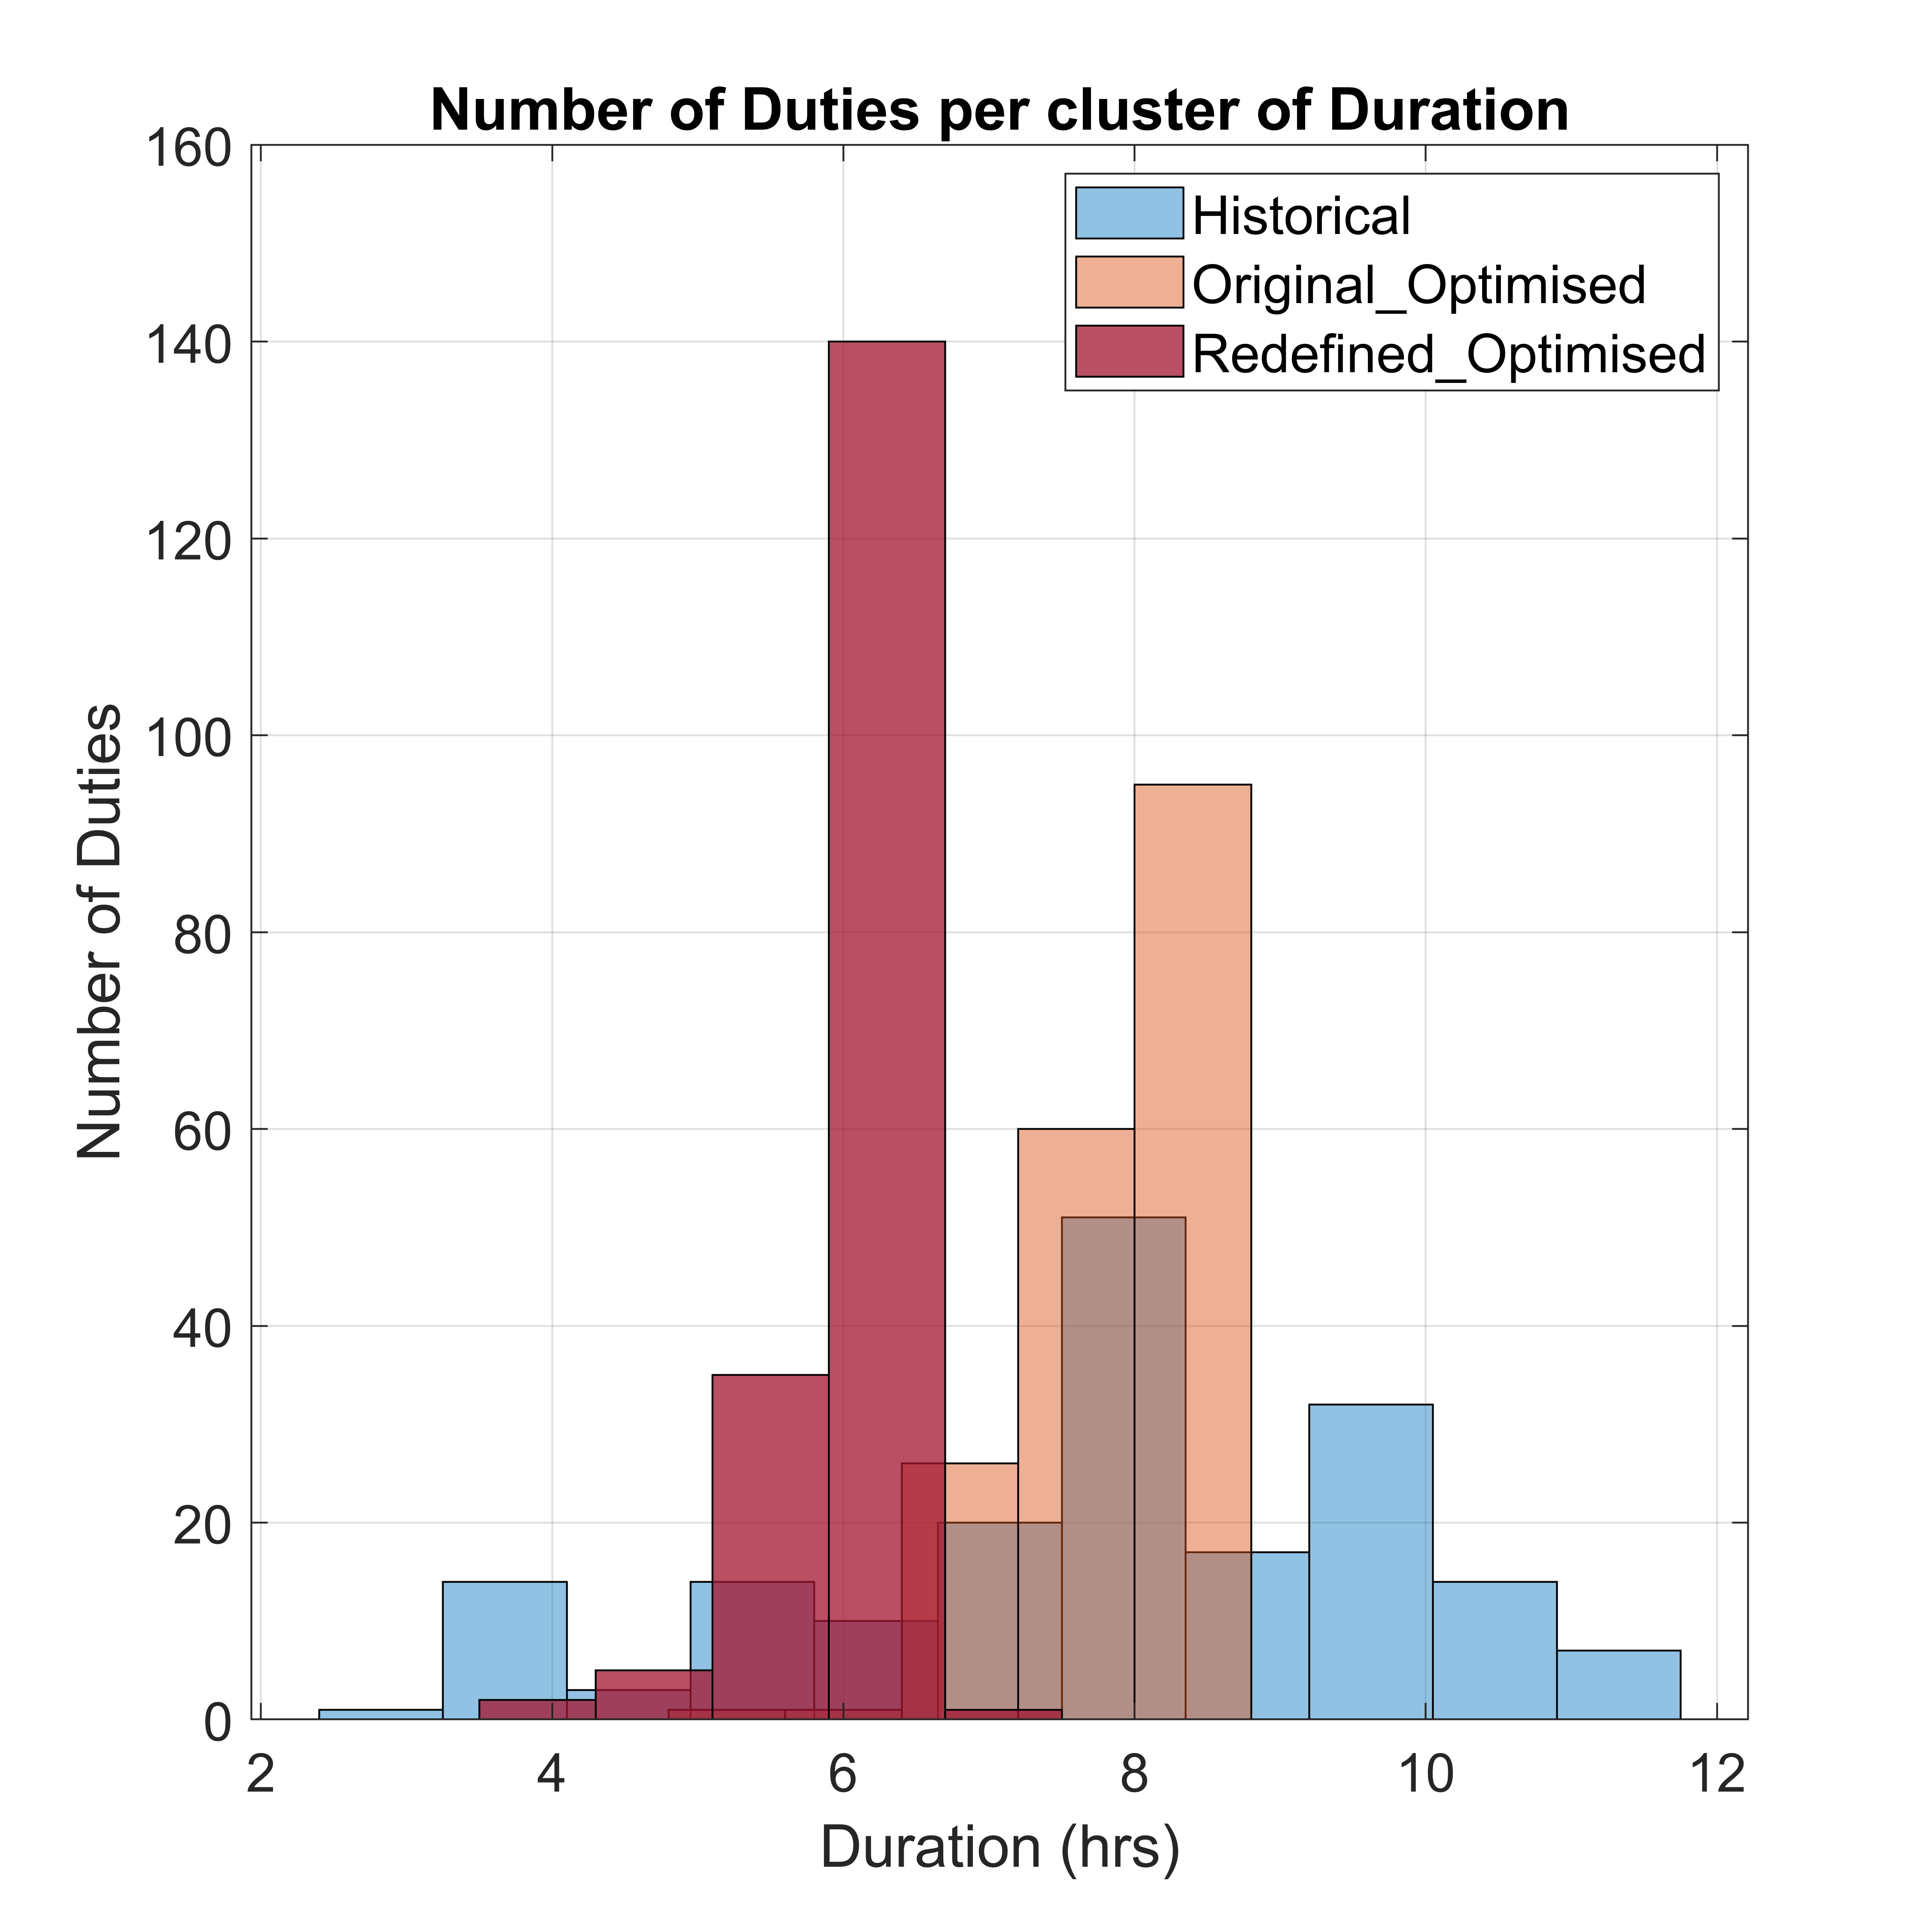
\includegraphics[width=0.46\linewidth]{[1] - chapter/Image Files/1-D2M1.png}
    }%\end{center}}%end of picture #2
    \caption{Illustrations of curves indicating our results.}%
    \label{fig:1-D2M1}%
\end{figure}
 
 %%%%%%%%%%%%%%%%%%%%%%%%%%%%%%%%%%%%%%%%%%%%%%%%%%%%%%%%%%%%%%%%%%%%%% Table %%%%%%%%%%%%%%%%%%%%%%%%%%%%%%%%%%%%%%%%%%%%%%%

\begin{table}[h]
\small
    \centering 
    \begin{tabular}{|l|c|c|c|c|}
        \hline
        \textbf{Schedule} & \multicolumn{3}{|c|}{ \textbf{Duties (HH:mm)}} & \textbf{Total Time}  \\
        \hline
         & \texttt{Average} &  \texttt{Minimum} & \texttt{Makespan} & \\
        \hline
        Historical  & 07:50 & 02:50 & 11:50 & 1,435:22 \\
        \hline
        Historical\_Optimised   & 07:50 & 05:15 & 08:25 & 1,435:22 \\
        \hline
        Redefined\_Optimised   & 06:06 & 03:55 & 07:27 & 1,118:58 \\
        \hline
    \end{tabular}%
    \medbreak
\end{table}
 
\vspace{\baselineskip}
\noindent
Observing the Histogram chart in Figure \ref{fig:1-D2M1}(b), we can see that long lasting shifts have been reduced down to duty lengths which are at the very least, smaller than 7 hours and 27 minutes which is the longest lasting shift (i.e. makespan). The majority of the workload has been assigned to such shifts lasting longer than 6 hours but also generally below the 7 hour mark. With respect to the makespan we see a \textbf{36\% reduction} compared to the historical instance.

\vspace{\baselineskip}
\noindent
The duty that pushes the makespan up to the 07:27 mark occurs only once, and the reason behind its increased duration relative to the bulk of shorter-lasting duties is because it holds the longest lasting block of 6 hours and 35 minutes. As a result, we could argue that the effective makespan of the Redefined schedule is slightly lower in reality since the majority of the duties last approximately 6 and a half hours. Hence, practically the whole cohort of drivers would have to work for 6 and a half hours, except for a single driver that would have to perform the 7 hours and 27 minutes lasting duty.

\vspace{\baselineskip}
\noindent
In terms of encapsulating the performance of generated schedule in a more concrete manner we list the following table outlining how the optimised schedule fairs against our two evaluation criteria:

%%%%%%%%%%%%%%%%%%%%%%%%%%%%%%%%%%%%%%%%%%%%%%%%%%%%%%%%%%%%%%%%%%%%%% Table %%%%%%%%%%%%%%%%%%%%%%%%%%%%%%%%%%%%%%%%%%%%%%%

\begin{table}[h]
\small
    \centering 
\begin{tabular}{c|c|c}
        \textbf{Schedule} & \textbf{Makespan Reduction (\%)} & Mean Deviation-\textbf{Reduction (\%)} \\
        \hline
         Historical\_Optimised & 28\% & 72\% \\
        \hline
         Redefined\_Optimised  & 36\% & 78\% \\ 
\end{tabular}
\end{table}

\vspace{\baselineskip}
\noindent
Comparing the optimised schedules that are created from the Historical and Redefined Instances respectively we see that as expected there is a further reduction of 8\% in the makespan of the Redefined schedule, and also the Redefined schedule has a 6\% lower standard deviation, capturing the fact that it is even more uniform than the Historical schedule. 

%%%%%%%%%%%%%%%%%%%%%%%%%%%%%%%%%%%%%%%%%%%%%%%%%%%%%%%%%%%%%%%%%%%%%%%%%%%%%%% sub-SECTION %%%%%%%%%%%%%%%%%%%%%%%%%%%%%%%%%%%%%%%%%%%%%%%%%%%%%%%%%%%%%%%%%%%%%%%%%%%%%%

\subsection*{Evaluation - Optimising Starting Time Cluster Instance}
As a final experiment on the Makespan Scheduling model we break our problem into separate instances that are designed to resemble the observation made through analysing the dataset\footnote{The \texttt{starting-time} analysis of the dataset mentioned is presented in detail in Appendix \ref{subsection: Appendix Starting times} for interested readers.} concerning the fact that duties tend to start in \textbf{wave}-like clusters. This observation is an important, design parameter that needs to be taken into serious consideration, as it automatically renders any results that we are able to obtain more \textit{practically oriented} and easier to realise from the perspective of Royal Mail. As outlined in Section \ref{section: Wave Instances - Data} we split our dataset into three autonomous sub-problems and we once more run the Makespan Scheduling model.

%%%%%%%%%%%%%%%%%%%%%%%%%%%%%%%%%%%%%%%%%%%%%%%%%%%%%%%%%%%%%%%%%%%%%% Table %%%%%%%%%%%%%%%%%%%%%%%%%%%%%%%%%%%%%%%%%%%%%%%

\begin{table}[h]
\small
    \centering 
    \begin{tabular}{|l|c|c|c|c|c|c|c|}
        \hline
        \textbf{Schedule} & \multicolumn{2}{|c|}{ \textbf{Characteristics}} & \multicolumn{3}{|c|}{ \textbf{Duties (HH:mm)}} & \textbf{Total Time}  \\
        \hline
        & \texttt{Duties} & \texttt{Blocks} & \texttt{Average} &  \texttt{Minimum} & \texttt{Makespan} & \\
        \hline
        Historical\_Optimised & 183 & 462  & 07:50 & 05:15 & 08:25 & 1,435:22 \\
        \hline
        Morning\_Optimised & 59 & 114 & 06:46 & 00:00 & 08:25 & 393:40 \\
        \hline
        Afternoon\_Optimised & 61 & 145 & 07:32 & 03:25 & 07:19 & 444:53 \\
        \hline
        Night\_Optimised & 63 & 203 & 09:27 & 08:40 & 09:30 & 596:34 \\
        \hline
    \end{tabular}%
    \medbreak
\end{table}

%%%%%%%%%%%%%%%%%%%%%%%%%%%%%%%%%%%%%%%%%%%%%%%%%%%%%%%%%%%%%%%%%%%%%%%%%%%%%%% Figure %%%%%%%%%%%%%%%%%%%%%%%%%%%%%%%%%%%%%%%%%%%%%%%%%%%%%%%%%%%%%%%%%%%%%%%%%%%%%%

\begin{figure}
\minipage{0.32\textwidth}
\subfloat[Morning]{%\begin{center}
  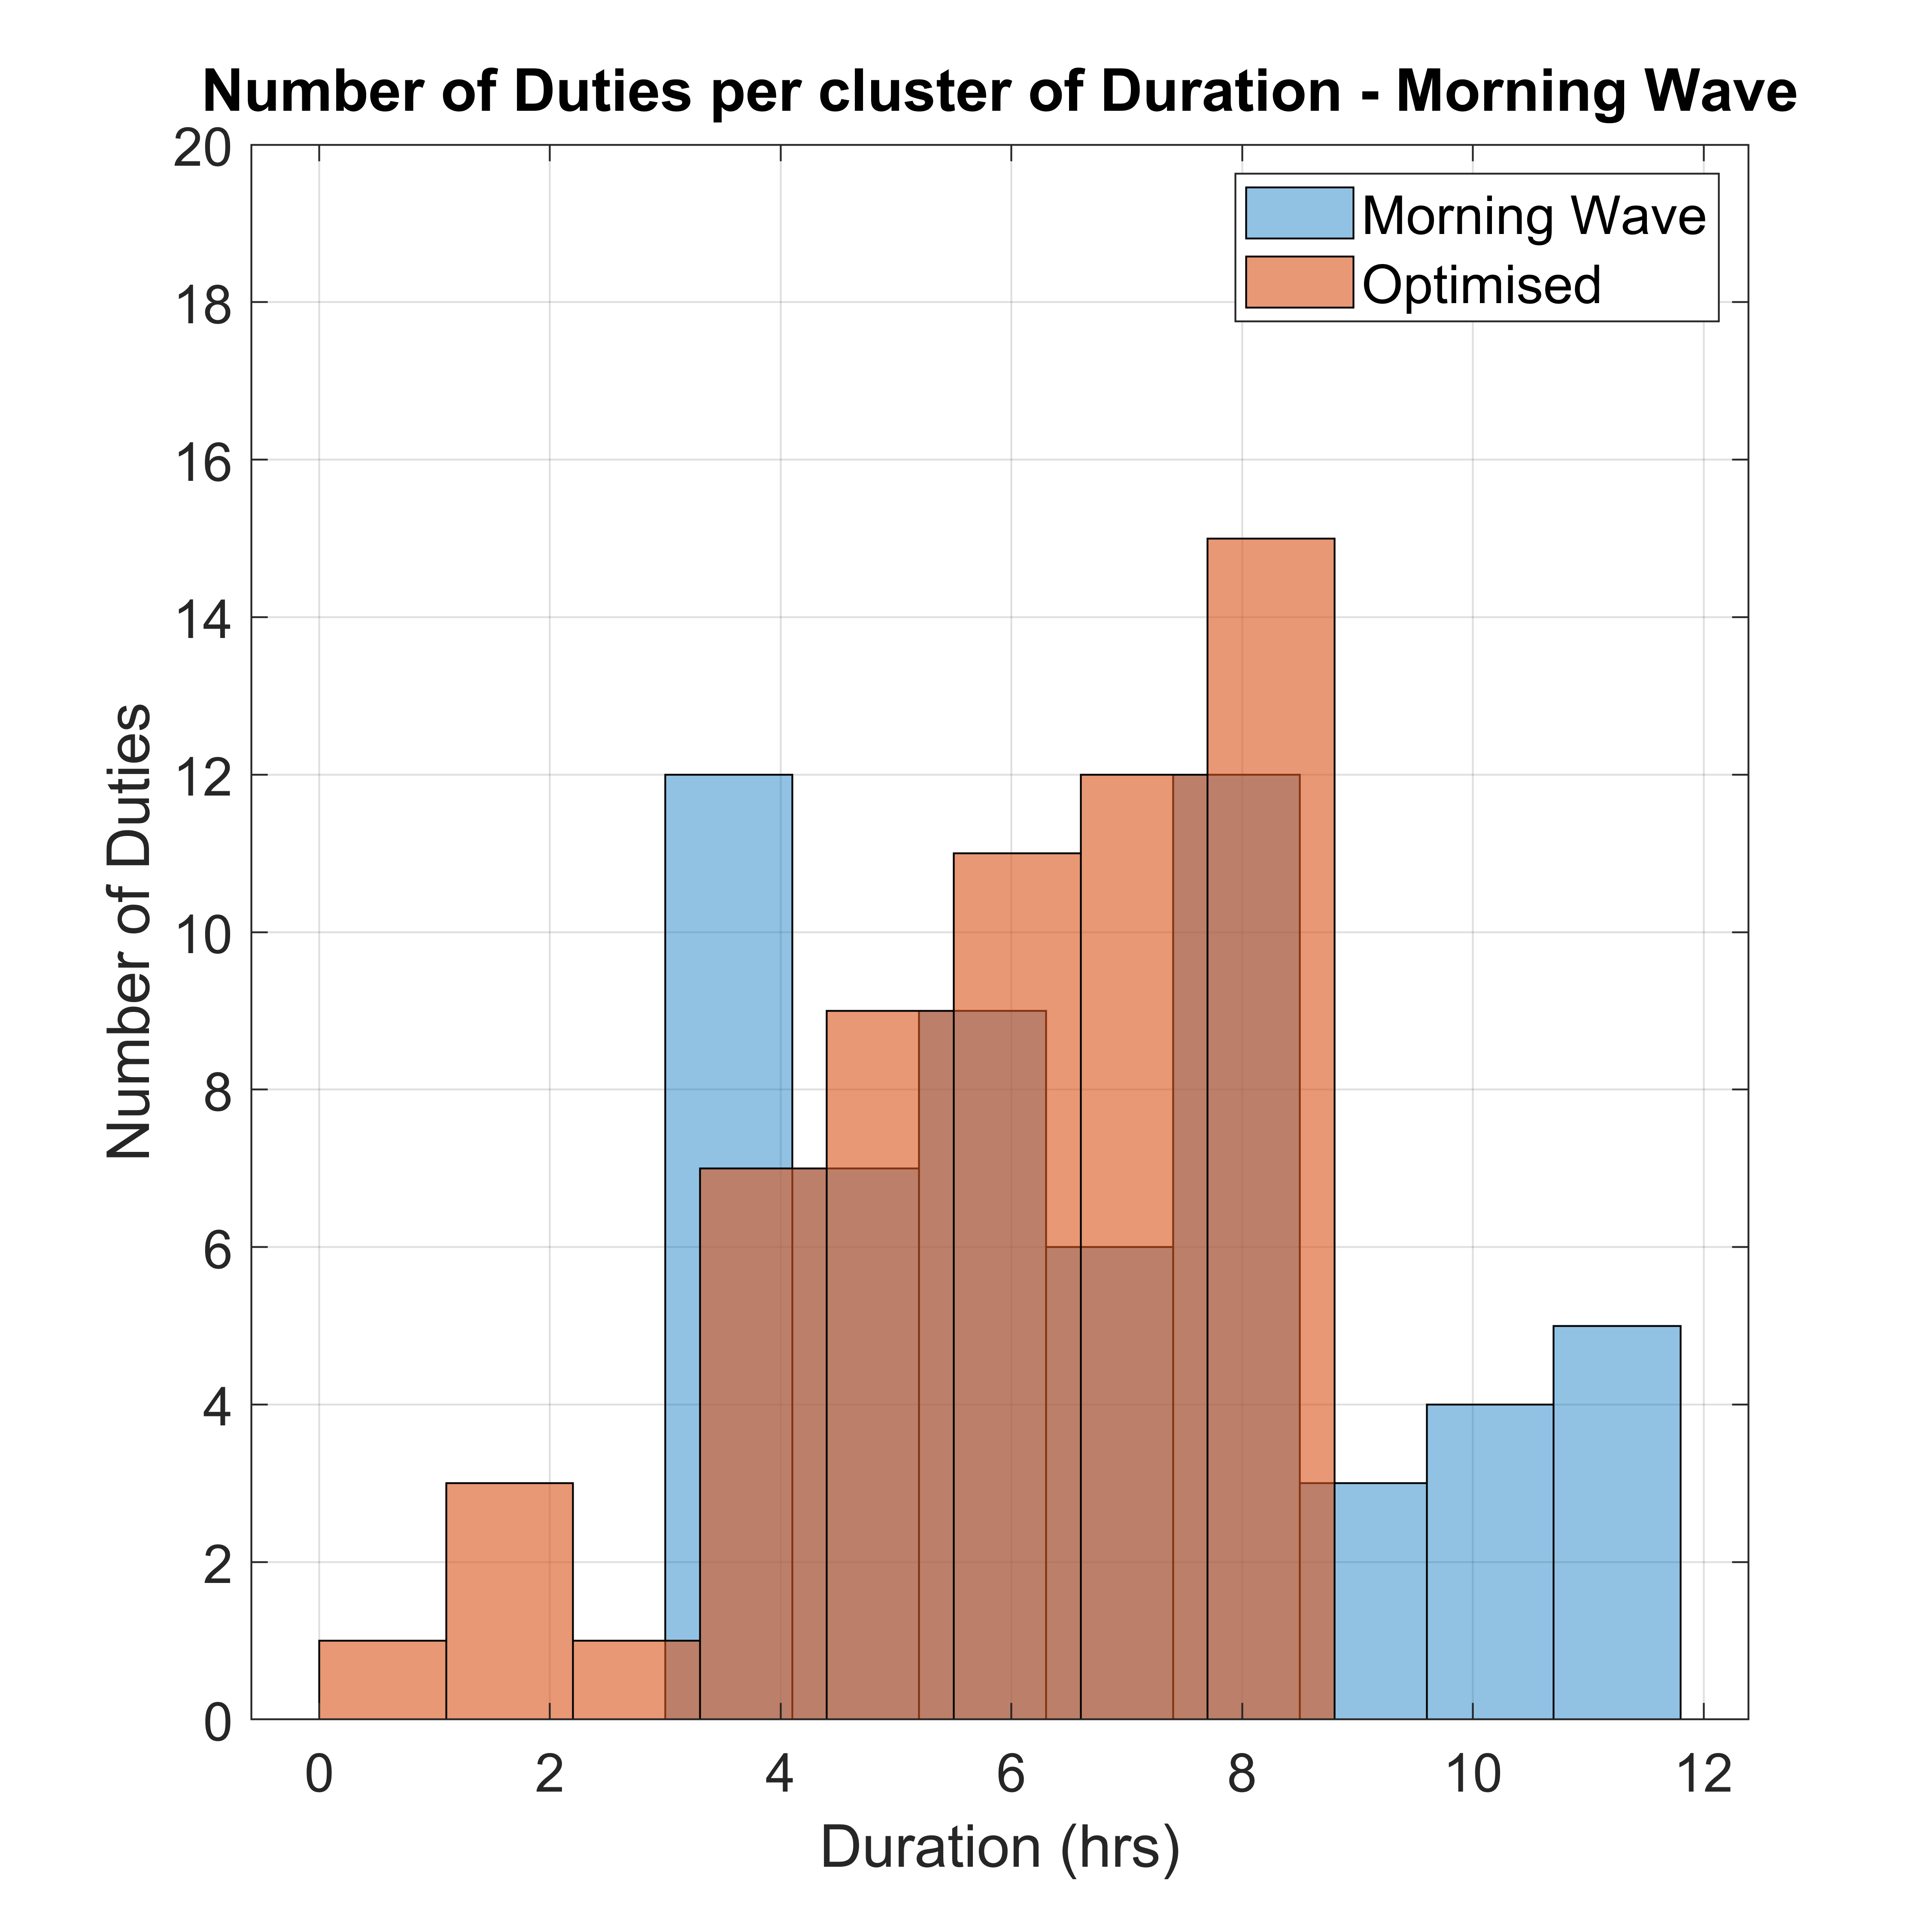
\includegraphics[width=\linewidth]{[2] - chapter/Image Files/morning.png}}
\endminipage\hfill
\minipage{0.32\textwidth}
\subfloat[Afternoon]{%\begin{center}
  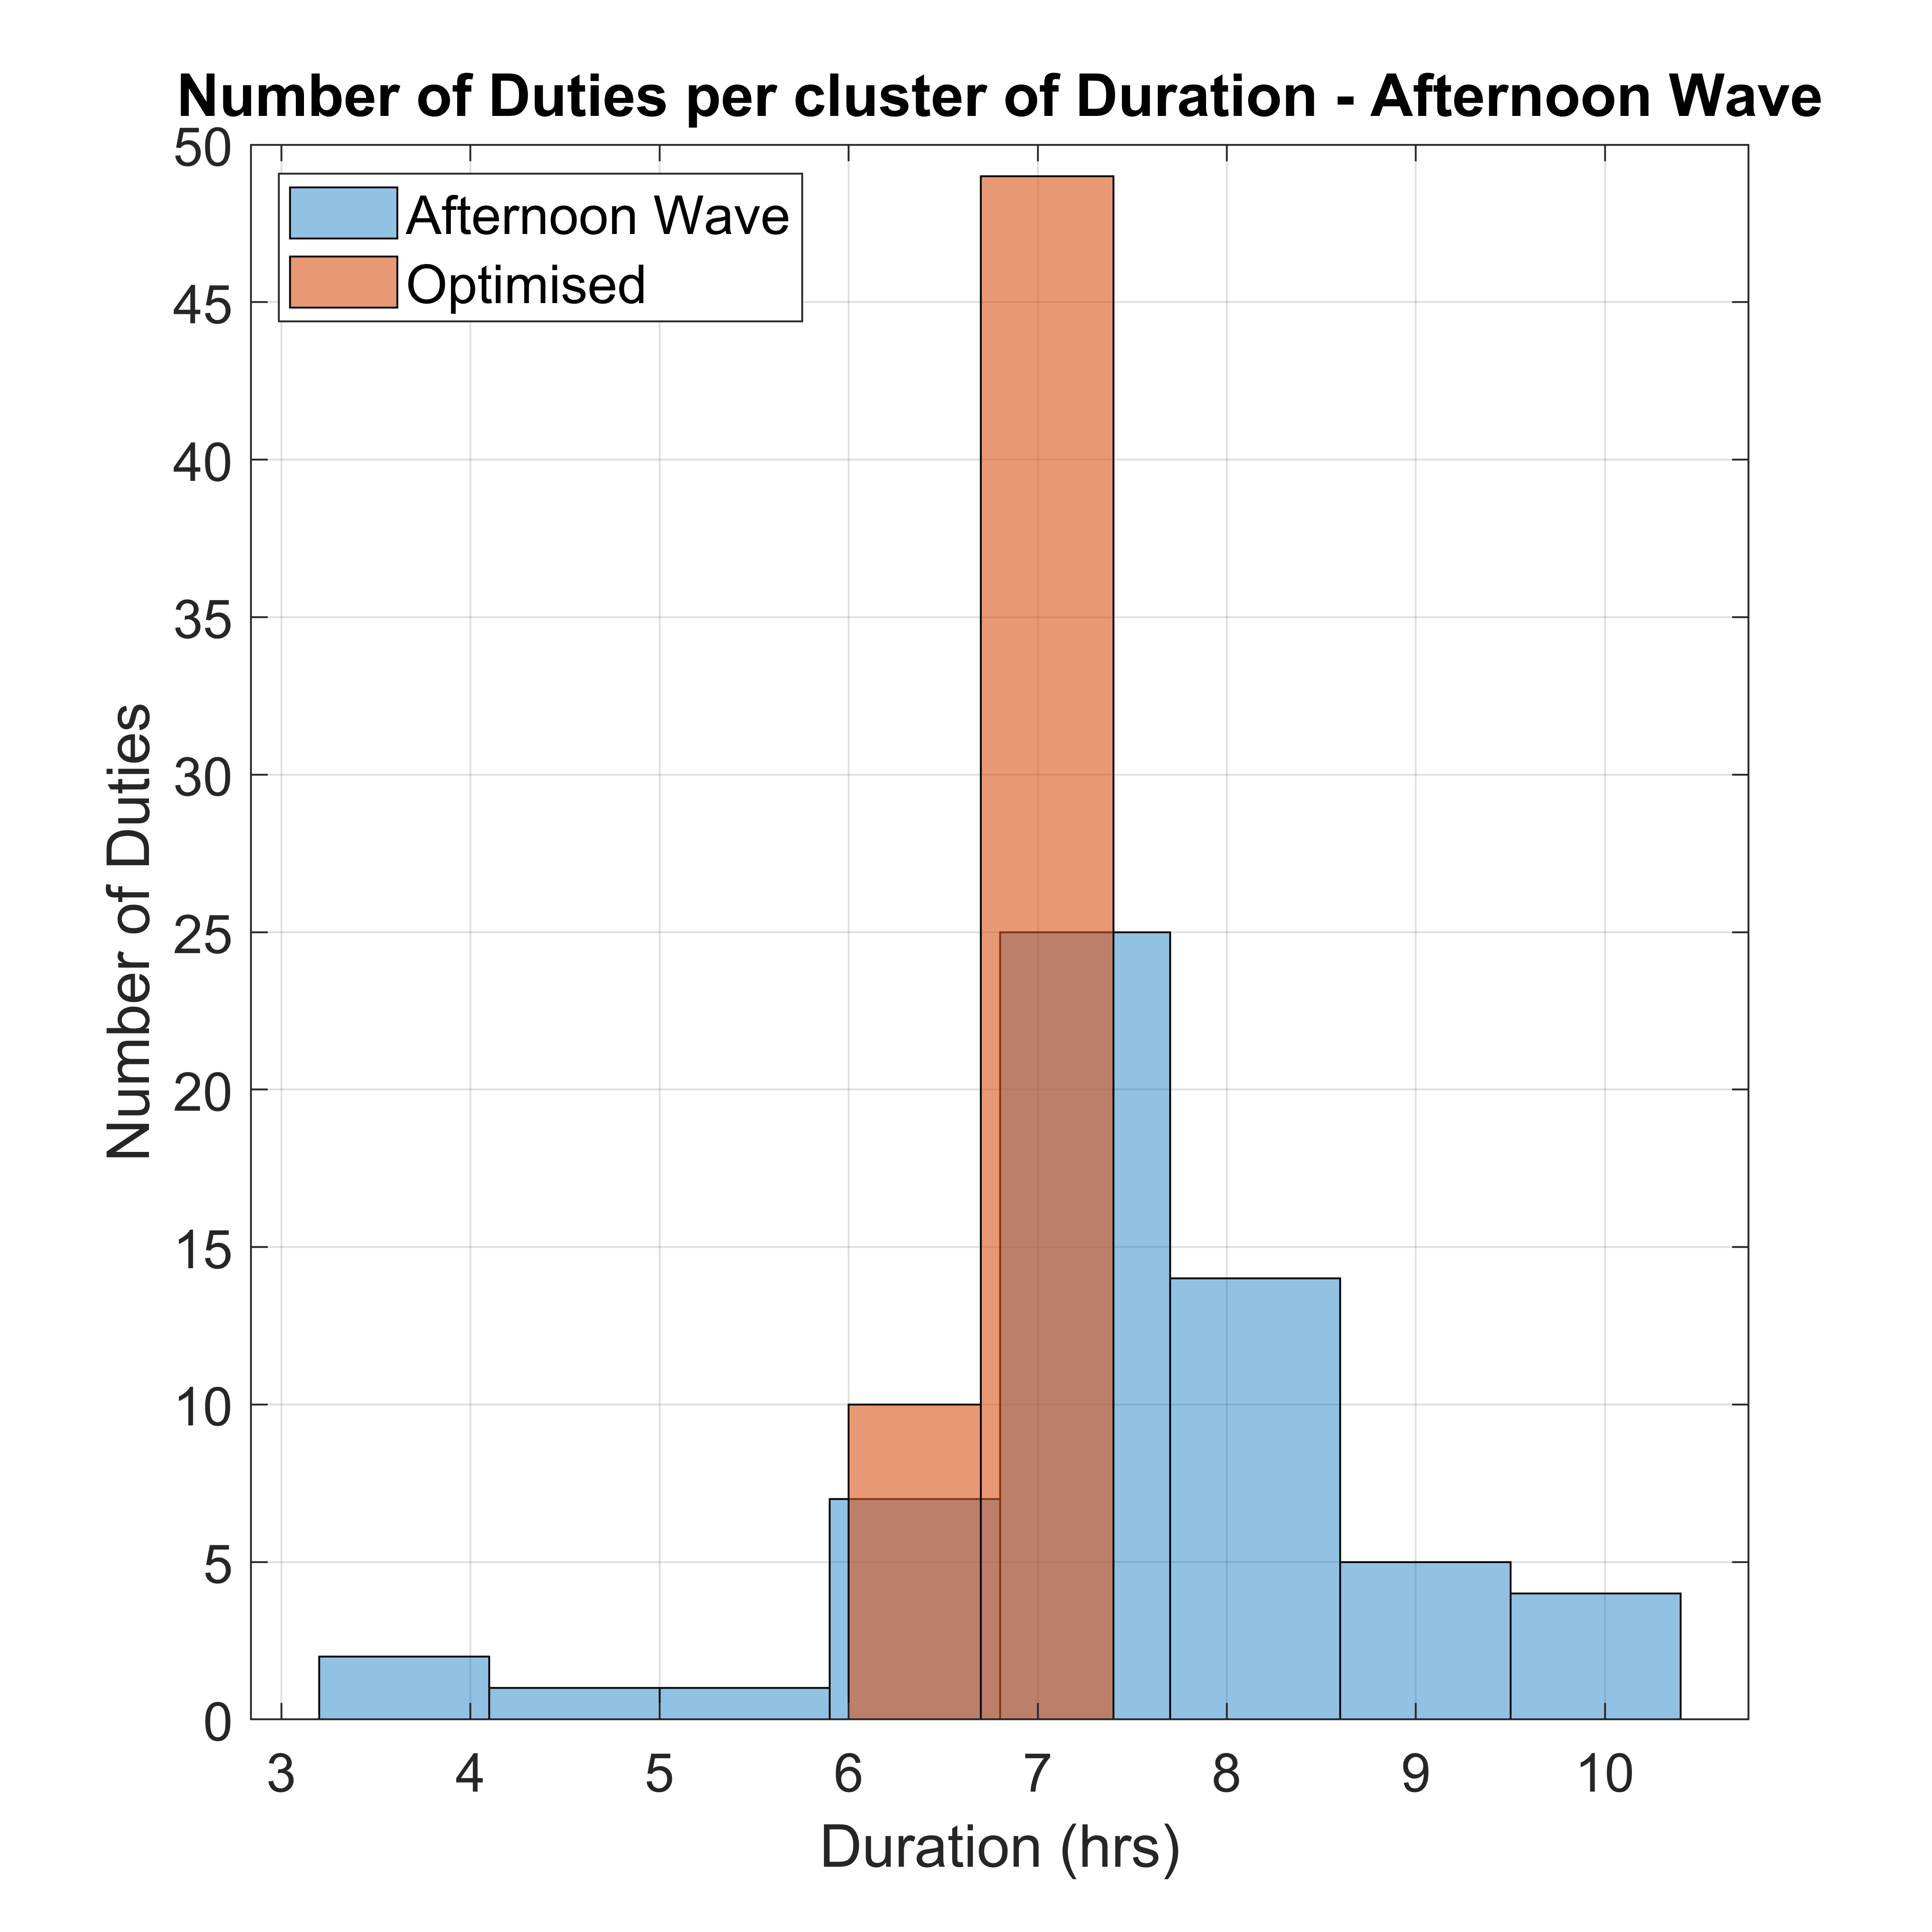
\includegraphics[width=\linewidth]{[2] - chapter/Image Files/afternoon.png}}
  
\endminipage\hfill
\minipage{0.32\textwidth}%
\subfloat[Night]{%\begin{center}
  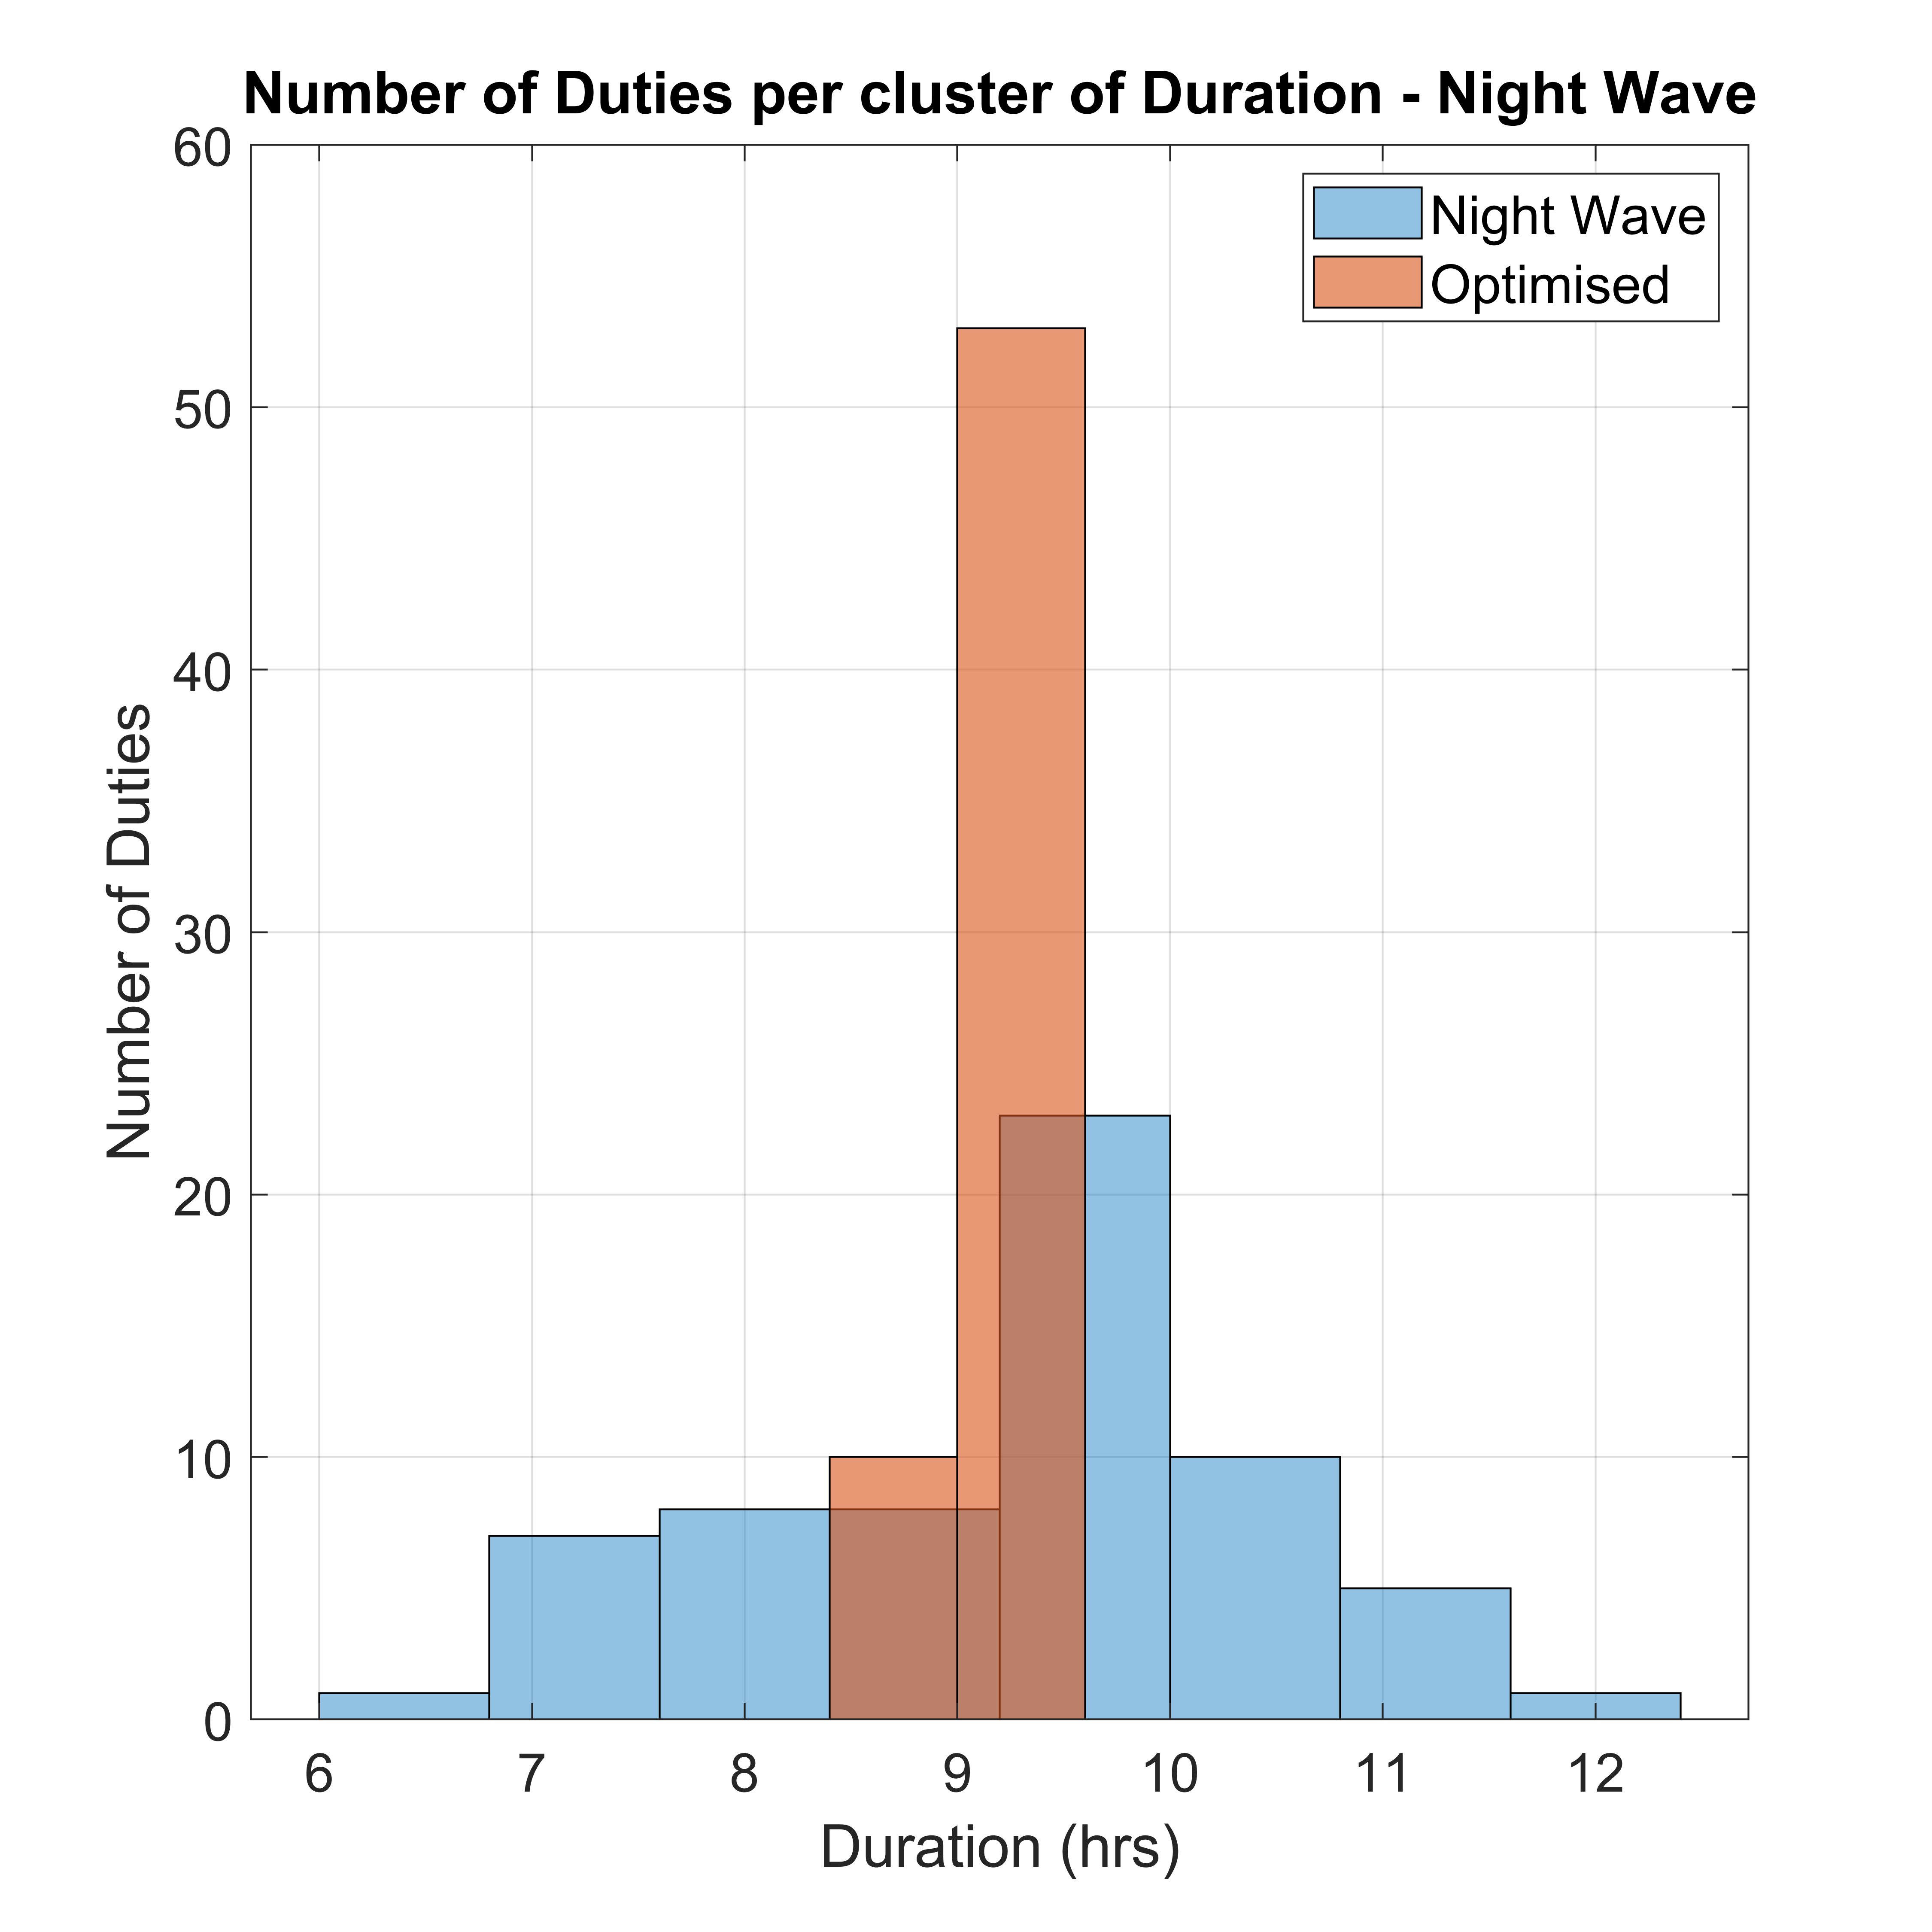
\includegraphics[width=\linewidth]{[2] - chapter/Image Files/night.png}}
 
\endminipage

\caption{The effects of Makespan Scheduling when considering our problem in Wave Instances.}
\label{fig: Wave Makespan Scheduling}
\end{figure}

\vspace{\baselineskip}
\noindent
The effects of re-organising our problem in such a fashion can be observed in Figure \ref{fig: Wave Makespan Scheduling}. Upon splitting our data into the three wave instances (\texttt{morning, afternoon, night})\footnote{The instances are listed in detail in Appendix \ref{subsection: redefine appexnix}} one can see that overall, the wave sub-instances do not consistently behave either better or worse than the schedule of the whole dataset seen previously in Figure \ref{fig:1-D1M1}(b). More specifically, in the \texttt{morning, afternoon} waves we can create schedules with a \textit{makespan} of around or below the makespan of the whole instance at the \textbf{08:25} mark, hence corroborating the fact that in an ideal schedule for the whole instance, the majority of duties should be of length below the 8 and a half hours mark obtained previously.

\vspace{\baselineskip}
\noindent
It is only in the \texttt{night} wave that we observe a sub-optimal makespan, relative to the other two. The \texttt{night} wave's makespan is beyond the 08:25 hour mark at 9 and a half hours. A sound argument behind this sub-optimal performance is to observe that the \texttt{night} wave has considerably more overall labor time to allocate than the other two instances. Moreover, it only has at most four more duties to allocate that time to, compared to the other two instances. Hence, the combination of more time to be scheduled and the limit amount of flexibility provided by the small amount of extra duties that the model has at its disposal to allocate that additional time to, lead to this sub-par performance with respect to the makespan.

\vspace{\baselineskip}
\noindent
On the other hand, the reason behind the great performance of our model in the \texttt{afternoon} instance could be zeroed down to the fact that the \texttt{afternoon} wave has the largest timespan out of the three waves (09:00-16:00), as can be seen in Table \ref{table:Starting Waves}, of Appendix \ref{subsection: Appendix Starting times}. Given, that it has a drastically bigger timespan, in fact equal to the sum of the other two instances, it might prove slightly easier to assign very late and very early starting duties since there will be more flexibility due this increased timespan.

\vspace{\baselineskip}
\noindent
Finally, we can see in Figure \ref{fig: Wave Makespan Scheduling}(a) that although the \texttt{morning} wave performs respectably with respect to its makespan, it lacks in its uniformity of the schedule compared to the other two wave instances, which enjoy a much tighter bandwidth. The non-optimised historical morning wave instance that our model receives as input could be identified as the cause for this lack of uniformity. More specifically, \ref{fig: Wave Makespan Scheduling}(a)-(c) we can see that the historical input instance for the \texttt{morning} is the least uniform out of the three. More importantly, it is \textit{right-skewed} when compared to the other two, hinting at the existence of numerous shorter-lasting shifts. As a result, our model is largely struggling to allocate the redistributed load from the longer lasting shifts to these shorter-lasting due to their small durations.  

\vspace{\baselineskip}
\noindent
These individual findings for each wave sub-instance justify the fact that the most frequently occurring duties in the whole dataset tend to have a duration between 6-8 hours. In addition, it is the shifts of the \texttt{night} wave, which contain the biggest portion of schedulable time, that end up contributing to pushing the makespan beyond 6 hours up to the 08:25 mark. 

\vspace{\baselineskip}
\noindent
All in all, by approximating the real-world through adding such constraints to our problem that make it more realistic in terms of its ease of implementation, for our Industrial Liaison, we have determined that the efficiency of our schedules is \textbf{not} significantly \textbf{compromised}. The \textit{makespan}, of the optimal schedule compared to that of the historical one is \textbf{equal or smaller} for two of the three waves. In addition, the optimised schedules are much more \textbf{uniform} than their historical equivalent, as seen in the table below\footnote{Each wave-optimised schedule is compared with its wave sub-instance for the table's evaluation criteria. Effectively, for each chart of Figure \ref{fig: Wave Makespan Scheduling} we compare the optimised schedule with the input wave instance.}:

%%%%%%%%%%%%%%%%%%%%%%%%%%%%%%%%%%%%%%%%%%%%%%%%%%%%%%%%%%%%%%%%%%%%%% Table %%%%%%%%%%%%%%%%%%%%%%%%%%%%%%%%%%%%%%%%%%%%%%%

\begin{table}[h]
\small
    \centering 
\begin{tabular}{l|c|c}
        \textbf{Schedule} & \textbf{Makespan Reduction (\%)} & Mean Deviation-\textbf{Reduction (\%)} \\
        \hline
         Historical\_Optimised & 28\% & 72\% \\
        \hline
         Morning\_Optimised  & 28\% & 14\% \\ 
         \hline
         Afternoon\_Optimised  & 29\% & 76\% \\ 
         \hline
         Night\_Optimised  & 19\% & 80\% \\ 
\end{tabular}
\end{table}

%%%%%%%%%%%%%%%%%%%%%%%%%%%%%%%%%%%%%%%%%%%%%%%%%%%%%%%%%%%%%%%%%%%%%%%%%%%%%%%SECTION%%%%%%%%%%%%%%%%%%%%%%%%%%%%%%%%%%%%%%%%%%%%%%%%%%%%%%%%%%%%%%%%%%%%%%%%%%%%%%
\section{Trade-off between Number of Completed Duties and Maximum Duty Length}
\label{section:minimise duties}
Upon proving that there exists significant room for improvement with respect to the historical schedule's makespan we re-examined the historical schedule to see if there are other aspects of it that could be improved. After a careful observation of the dataset we noticed that there are potentially too many duties in the historical schedule. Consequently, people have to work a lot to carry out all those duties. To remedy this, we attempt to minimise the number of duties that are required to complete the same amount of workload (i.e. same amount of blocks). 

\vspace{\baselineskip}
\noindent
Provided we are able to decrease the number of duties for the same amount of blocks, this would translate to people working less, since there would be less duties requiring completion. In practical terms this amounts to a transformation of our problem to a Bi-Objective Generalised Assignment Problem \cite{PRAKASH2010} since it aims to \textbf{minimise} the \textbf{maximum duty length}, while also \textbf{minimising} the \textbf{number of duties}. 

\vspace{\baselineskip}
\noindent
To solve this problem we need to develop an algorithm that will provide us with the Pareto Optimal points of the problem. Those points will represent Pareto Optimal schedules, and our Industrial Partners can evaluate each of those schedules to select the one that best fits their company policy requirements. We rely upon the formulation of the previous section but shift the focus of the minimisation problem onto minimising the number of duties that need to be operational to carry out the required tasks. We hypothesise that we can fix an upper threshold for the duty length ($L$). We hence assume that people have to work $L$ hours, and not any more than that. 

\vspace{\baselineskip}
\noindent
For the purposes of our solver that means that it can schedule duties that are only as long as that threshold. The solver hence, has at its disposal duties that are subject to this upper bound to and has to attempt to fit all the blocks inside of them. In practice this is enforced by creating a constraint that applies this upper bound restriction to the duties' lengths. We hence, take the minimisation of the duration out of the objective function of this problem but it remains in spirit as the secondary objective that we will attempt to minimise through our sensitivity analysis.

\vspace{\baselineskip}
\noindent
The variable $y_{i}$ contains a value that specifies the number of duties $i$ that are \textbf{required}. Similarly to the previous formulation binary variable $x_{i,j}$ dictates the assignment of a block $j$ to a duty $i$ and is equal to 1 if the atomic block $j \in B$ is assigned to duty $i \in D$, and 0 otherwise.

%%%%%%%%%%%%%%%%%%%%%%%%%%%%%%%%%%%%%%%%%%%%%%%%%%%%%%%%%%%%%%%%%%%%%%%%%%%%%%% Maths %%%%%%%%%%%%%%%%%%%%%%%%%%%%%%%%%%%%%%%%%%%%%%%%%%%%%%%%%%%%%%%%%%%%%%%%%%%%%%

\vspace{\baselineskip}
\begin{equation}
\label{equation: Minimise Duties}
\begin{aligned}
&\text{minimise}
& & \sum _{i=1}^m y_{i}  \\
& \text{subject to}
& & y_{i} \geq x_{i,j}  \;\;\; &\forall \; i \in D,\; j \in B\\   
& & &\sum _{i=1}^m x_{i,j} = 1 \;\;\; &\forall \; j \in B\\
%& & &\sum _{j=1}^n x_{i,j}p_{j} \leq f_{i}-s_{i} \;\;\; &\forall \; i \in D\\
& & &\sum _{j=1}^n x_{i,j}p_{j} \leq L \;\;\; &\forall \; i \in D\\
& & & y\geq 0  \\
& & & x_{i,j} \in  \{ 0,1 \} \;\;\; &\forall \; j \in B, \; i \in D\\
\end{aligned}
\end{equation}

\vspace{\baselineskip}
\noindent
The model minimises the number of active duties. The first constraint makes sure that a duty $i$ is counted as active if at least one of the $x_{i,j}$ is equal to 1. The second constraint makes sure that each atomic block is executed by one and only one duty. Finally, the third constraint makes sure that the contents of a duty do not exceed the maximum duty length threshold $L$. This maximum duty length is determined by the hyper-parameter $L$ that we supply as input to the model 36 times to complete the sensitivity analysis. 

%%%%%%%%%%%%%%%%%%%%%%%%%%%%%%%%%%%%%%%%%%%%%%%%%%%%%%%%%%%%%%%%%%%%%%%%%%%%%%% sub-SECTION %%%%%%%%%%%%%%%%%%%%%%%%%%%%%%%%%%%%%%%%%%%%%%%%%%%%%%%%%%%%%%%%%%%%%%%%%%%%%%

\subsection*{Evaluation}
\vspace{\baselineskip}
\noindent
Using this formulation we investigate the number of active duties that can be reduced for various levels of the maximum duty length. This investigation is carried out by conducting a sensitivity analysis, where we vary the hyper-parameter $L$ and measure the number of duties required. A particularly important threshold that we choose to focus on is that of setting \textit{L} equal to the maximum duty length observed in the historical schedule. This will allow us to determine the optimal number of duties that could have been used instead of the historically used 183 duties utilised by Royal Mail. 

%%%%%%%%%%%%%%%%%%%%%%%%%%%%%%%%%%%%%%%%%%%%%%%%%%%%%%%%%%%%%%%%%%%%%%%%%%%%%%% Figure %%%%%%%%%%%%%%%%%%%%%%%%%%%%%%%%%%%%%%%%%%%%%%%%%%%%%%%%%%%%%%%%%%%%%%%%%%%%%%

\begin{figure}%
    \centering
    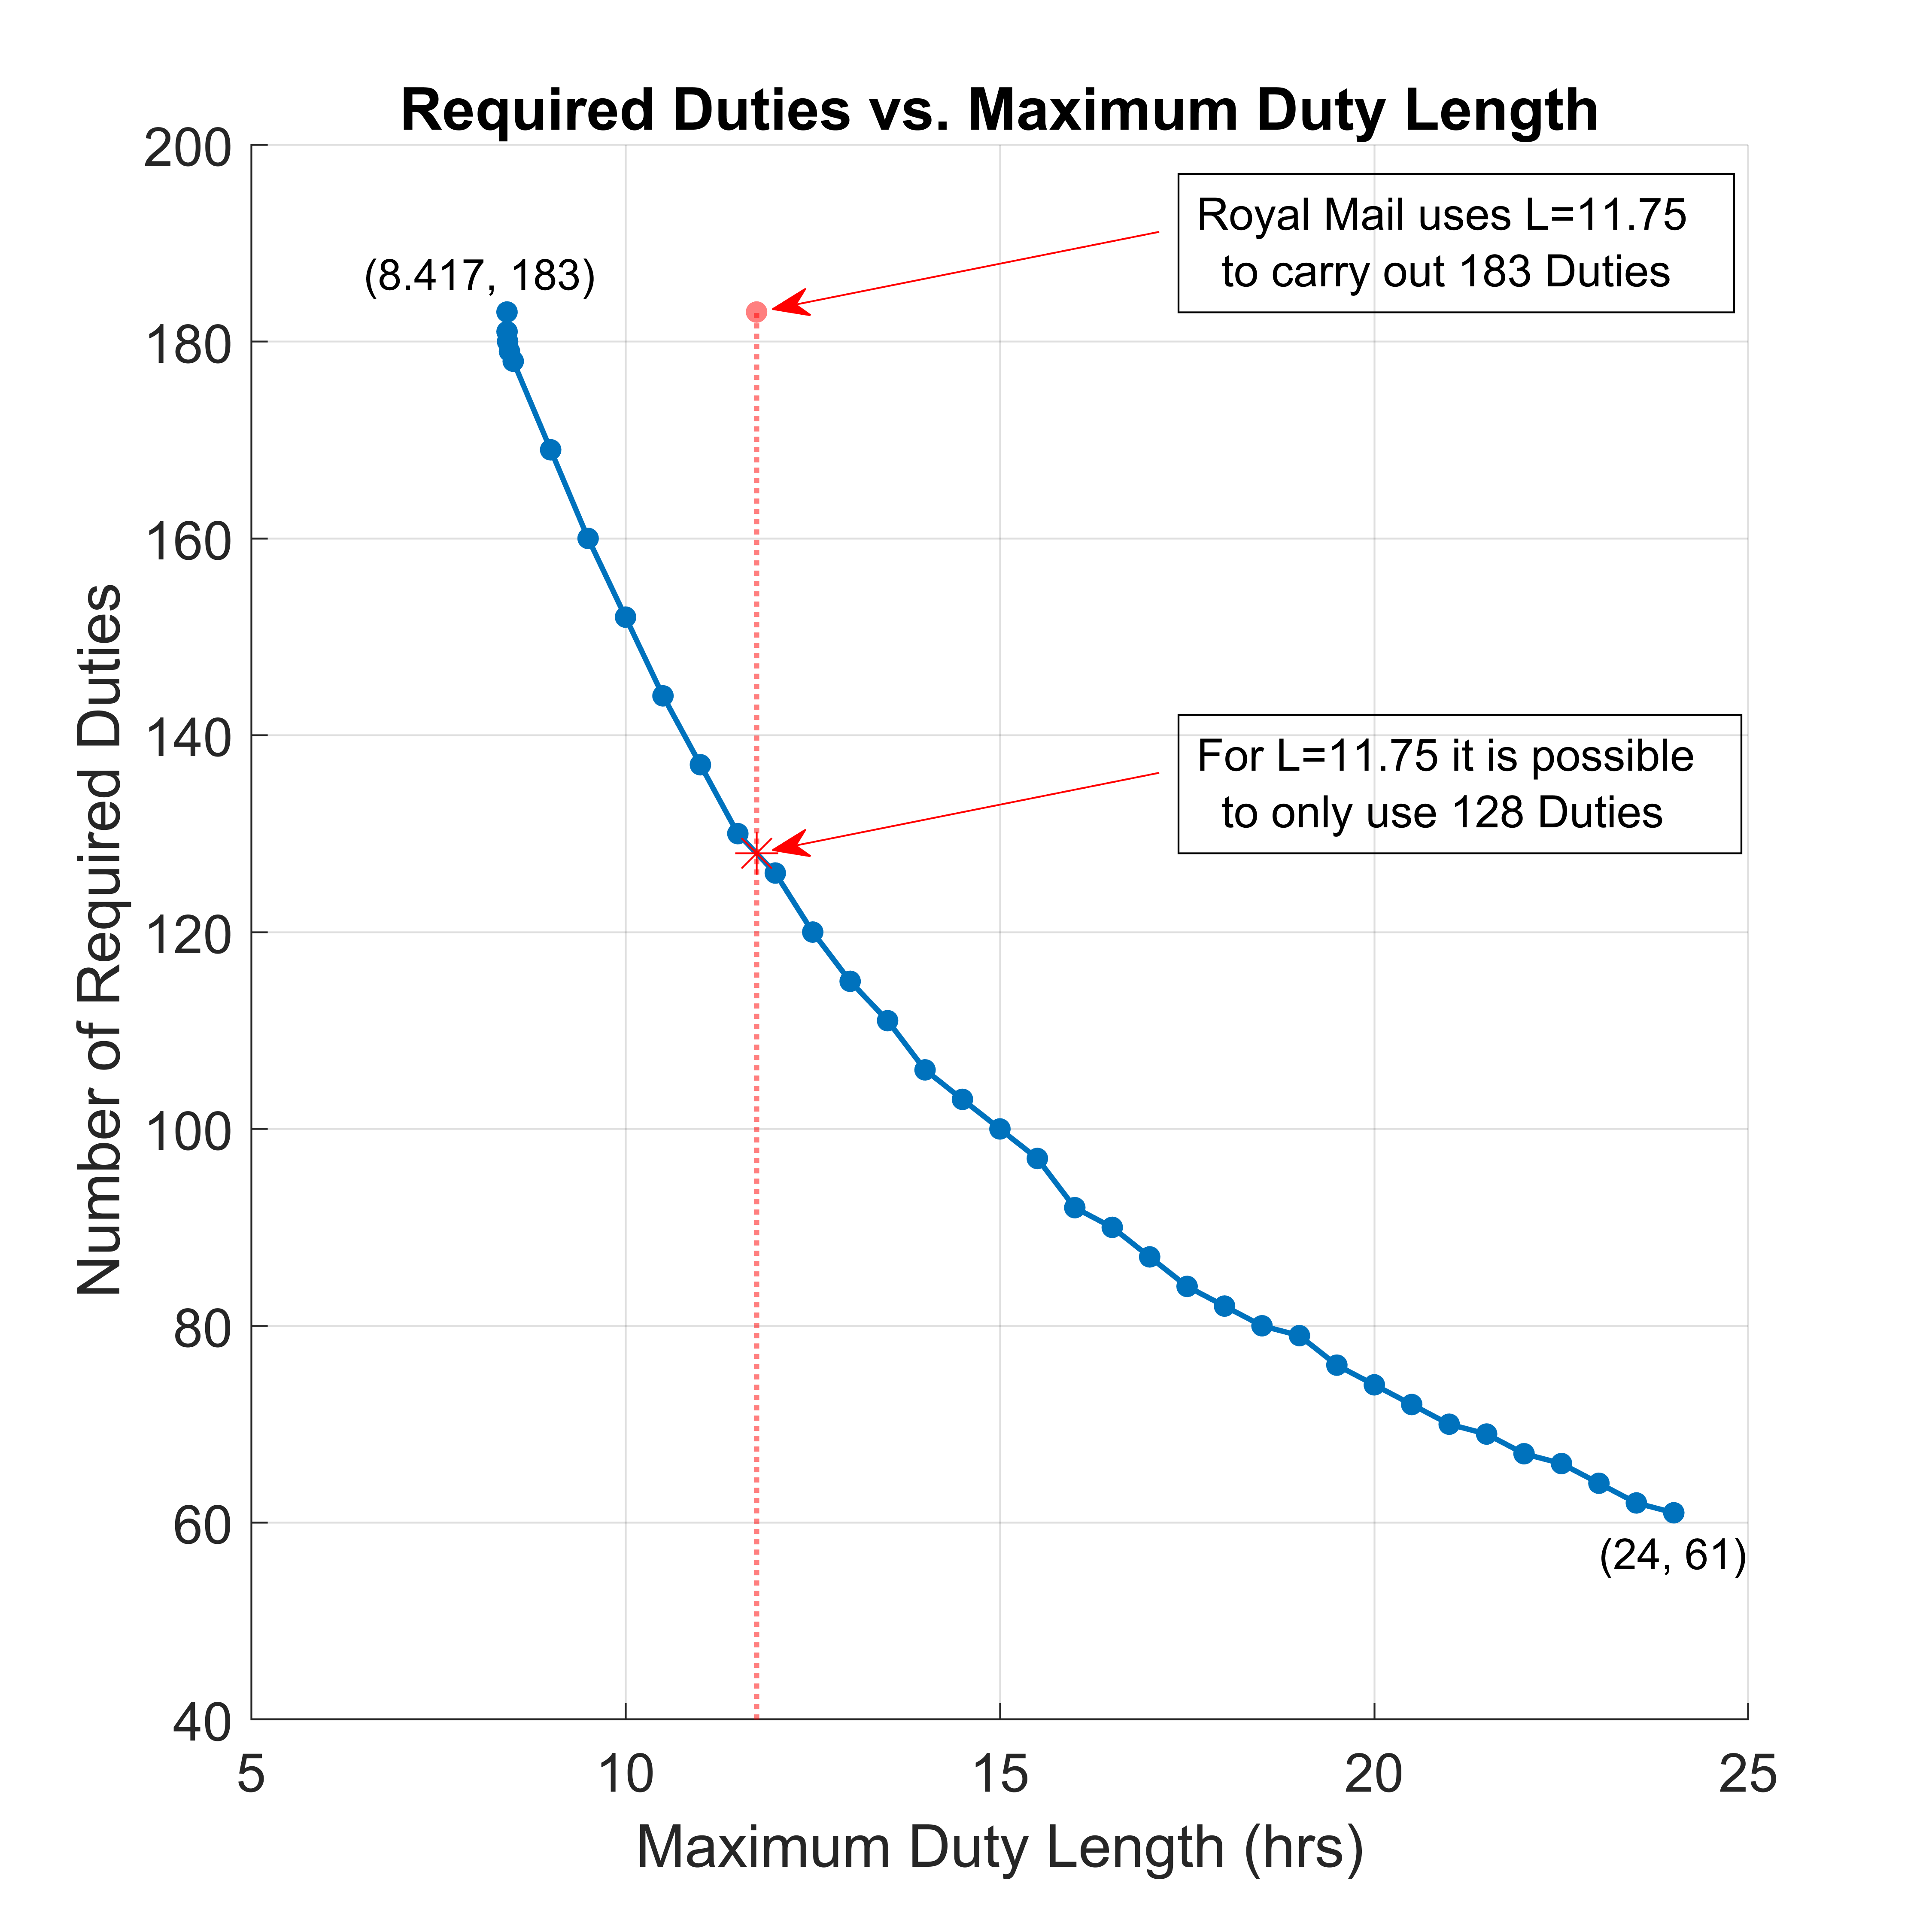
\includegraphics[width=0.46\linewidth]{[1] - chapter/Image Files/1-D1M2.png}
    \caption{Depicts the number of duties required as a function of the Maximum Duty Length varied in 30 minute intervals, up to an \textit{upper threshold} of \textbf{24 hours} per duty.}
    \label{fig:1-D1M2}
\end{figure}

%%%%%%%%%%%%%%%%%%%%%%%%%%%%%%%%%%%%%%%%%%%%%%%%%%%%%%%%%%%%%%%%%%%%%%%%%%%%%%% sub-SECTION %%%%%%%%%%%%%%%%%%%%%%%%%%%%%%%%%%%%%%%%%%%%%%%%%%%%%%%%%%%%%%%%%%%%%%%%%%%%%%

\subsubsection*{Qualitative Results}
In Figure \ref{fig:1-D1M2} we plot the result of the sensitivity analysis. In more detail, through utilising the principle of the Pareto front we computed the efficient frontier seen in Figure \ref{fig:1-D1M2} by applying algorithm (\ref{alg: Pareto}) 36 times\footnote{\label{Pareto}Seen in Section \ref{section: Pareto} of Chapter \ref{chapter: Background}} between a minimum and maximum \textit{L}. Hence, the trade-off curve shows the sensitivity analysis in its entirety applying the Pareto algorithm from a maximum \textit{L} of 24 hours down to a minimum \textit{L} of around 8 and half hours, that still provides a feasible schedule. Obviously, we cannot expect an individual to complete duty lasting 24 hours, however, we present the Pareto front to allow the flexibility for our industrial partner. Figure \ref{fig:1-D1M2} shows that if the maximum duty length increases the number of duties required decreases significantly. 



%%%%%%%%%%%%%%%%%%%%%%%%%%%%%%%%%%%%%%%%%%%%%%%%%%%%%%%%%%%%%%%%%%%%%%%%%%%%%%% sub-SECTION %%%%%%%%%%%%%%%%%%%%%%%%%%%%%%%%%%%%%%%%%%%%%%%%%%%%%%%%%%%%%%%%%%%%%%%%%%%%%%

\subsubsection*{Quantitative Results}
As mentioned before although it might not be directly reflected in equation (\ref{equation: Minimise Duties}) this is principally a Bi-Objective problem where the two objectives minimised are the maximum duty length (\textit{L}) and the number of duties. As result, on the left end of the curve one can see the value of \textit{L} for which the objective regarding the minimisation of \textit{L} is best satisfied. As observed in Figure \ref{fig:1-D1M2} that minimal value of \textit{L} is equal to 8.417 hours\footnote{Which amounts to 8 hours and 25 minutes.} and this allows us to complete all blocks in the original 183 duties. Hence, we have identified an optimisation opportunity since it is possible to allocate the same workload into a schedule with \textbf{shorter maximum lasting duty} compared to the historical practices. A careful observer will recognise that this exact finding was been seen in an earlier stage of this report. Namely, this value for the maximum duty length, coincides exactly with the value found for the Makespan of the optimal schedule in Section \ref{section:Makespan Scheduling-content}. Consequently, we can be sure that the schedule with $L=8.417 \text{ hours}$ is a Pareto optimal schedule that satisfies the minimisation of the maximum duty length objective of this problem.

\vspace{\baselineskip}
\noindent
Moreover, looking at the rest of the curve we can see that we have determined that we are able to reduce the amount of duties required significantly, as we increase hyper-parameter $L$. Using the \textit{L}-\textbf{threshold} of around 12 hours currently utilised by Royal Mail allows us to use a mere 128 duties compared to the 183 required by Royal Mail. This translates to a \textbf{30\%} reduction in the duties that need to be fulfilled for the same maximum duty length (\textit{L)}. Practically this means that if a small portion of the drivers is able to complete overtime duties (up to that 12 hours threshold) the remaining cohort of drivers would be able to work less since there would be less duties to be completed. 


\vspace{\baselineskip}
\noindent
The realisation that Royal Mail's current operating scenario is not on the Pareto frontier, is another indication that there is a substantial need for optimisation that will most likely lead to opportunities for cost cuts once Royal Mail places itself on the frontier. Taking into account the reality-based constraints that would constrict the provision of more efficient scheduling, we proceed to propose the most optimal but realistic schedule that Royal Mail can aim towards. That practical limit is founded in the fact that the maximum number of labor hours per day for an individual is a total of 13 hours as determined by EU rules\footnote{Seen in Appendix \ref{section: EU rules}}. If we proceed to utilise a maximum duty length $(L)$ of 13 hours the Pareto optimal schedule that we can achieve requires merely 115 duties to be completed. This would be a significant decrease over the 183 duties of the historical solution.

\vspace{\baselineskip}
\noindent
Finally, looking at the \textbf{theoretical optimal schedule} with respect to the other objective of this problem (i.e. minimal \textit{L}) we claim in theory we can do even better than a schedule with $L=8.417 \text{ hours}$. The most optimal schedule that we can hope to achieve is a schedule with a maximum duty length equal to that of the average duty duration of the input instance. That is because such a schedule would be equivalent to spreading the total schedulable hours equally to all 183 available duties. The historical schedules contained 183 duties with an average duty length 7 hours and 50 minutes, equivalent to 1435 hours and 22 minutes of total workload. We can see that the lowest feasible threshold for our maximum duty length in Figure \ref{fig:1-D1M2} is that of 8 hours and 25 minutes. This indicates that there an optimality gap between the ideal maximum duty length and the practical one. This is to be expected, due to the fact that the theoretical optimum could only be achieved if we neglect assumption (1) from Section \ref{section: 4.1}. In reality the atomic blocks in the input instance have an arbitrary size and hence we cannot obtain an exact fit of the blocks to all duties that sums to 7 hours and 50 minutes.

%%%%%%%%%%%%%%%%%%%%%%%%%%%%%%%%%%%%%%%%%%%%%%%%%%%%%%%%%%%%%%%%%%%%%%%%%%%%%%% Figure %%%%%%%%%%%%%%%%%%%%%%%%%%%%%%%%%%%%%%%%%%%%%%%%%%%%%%%%%%%%%%%%%%%%%%%%%%%%%%

\begin{figure}%
    \centering
    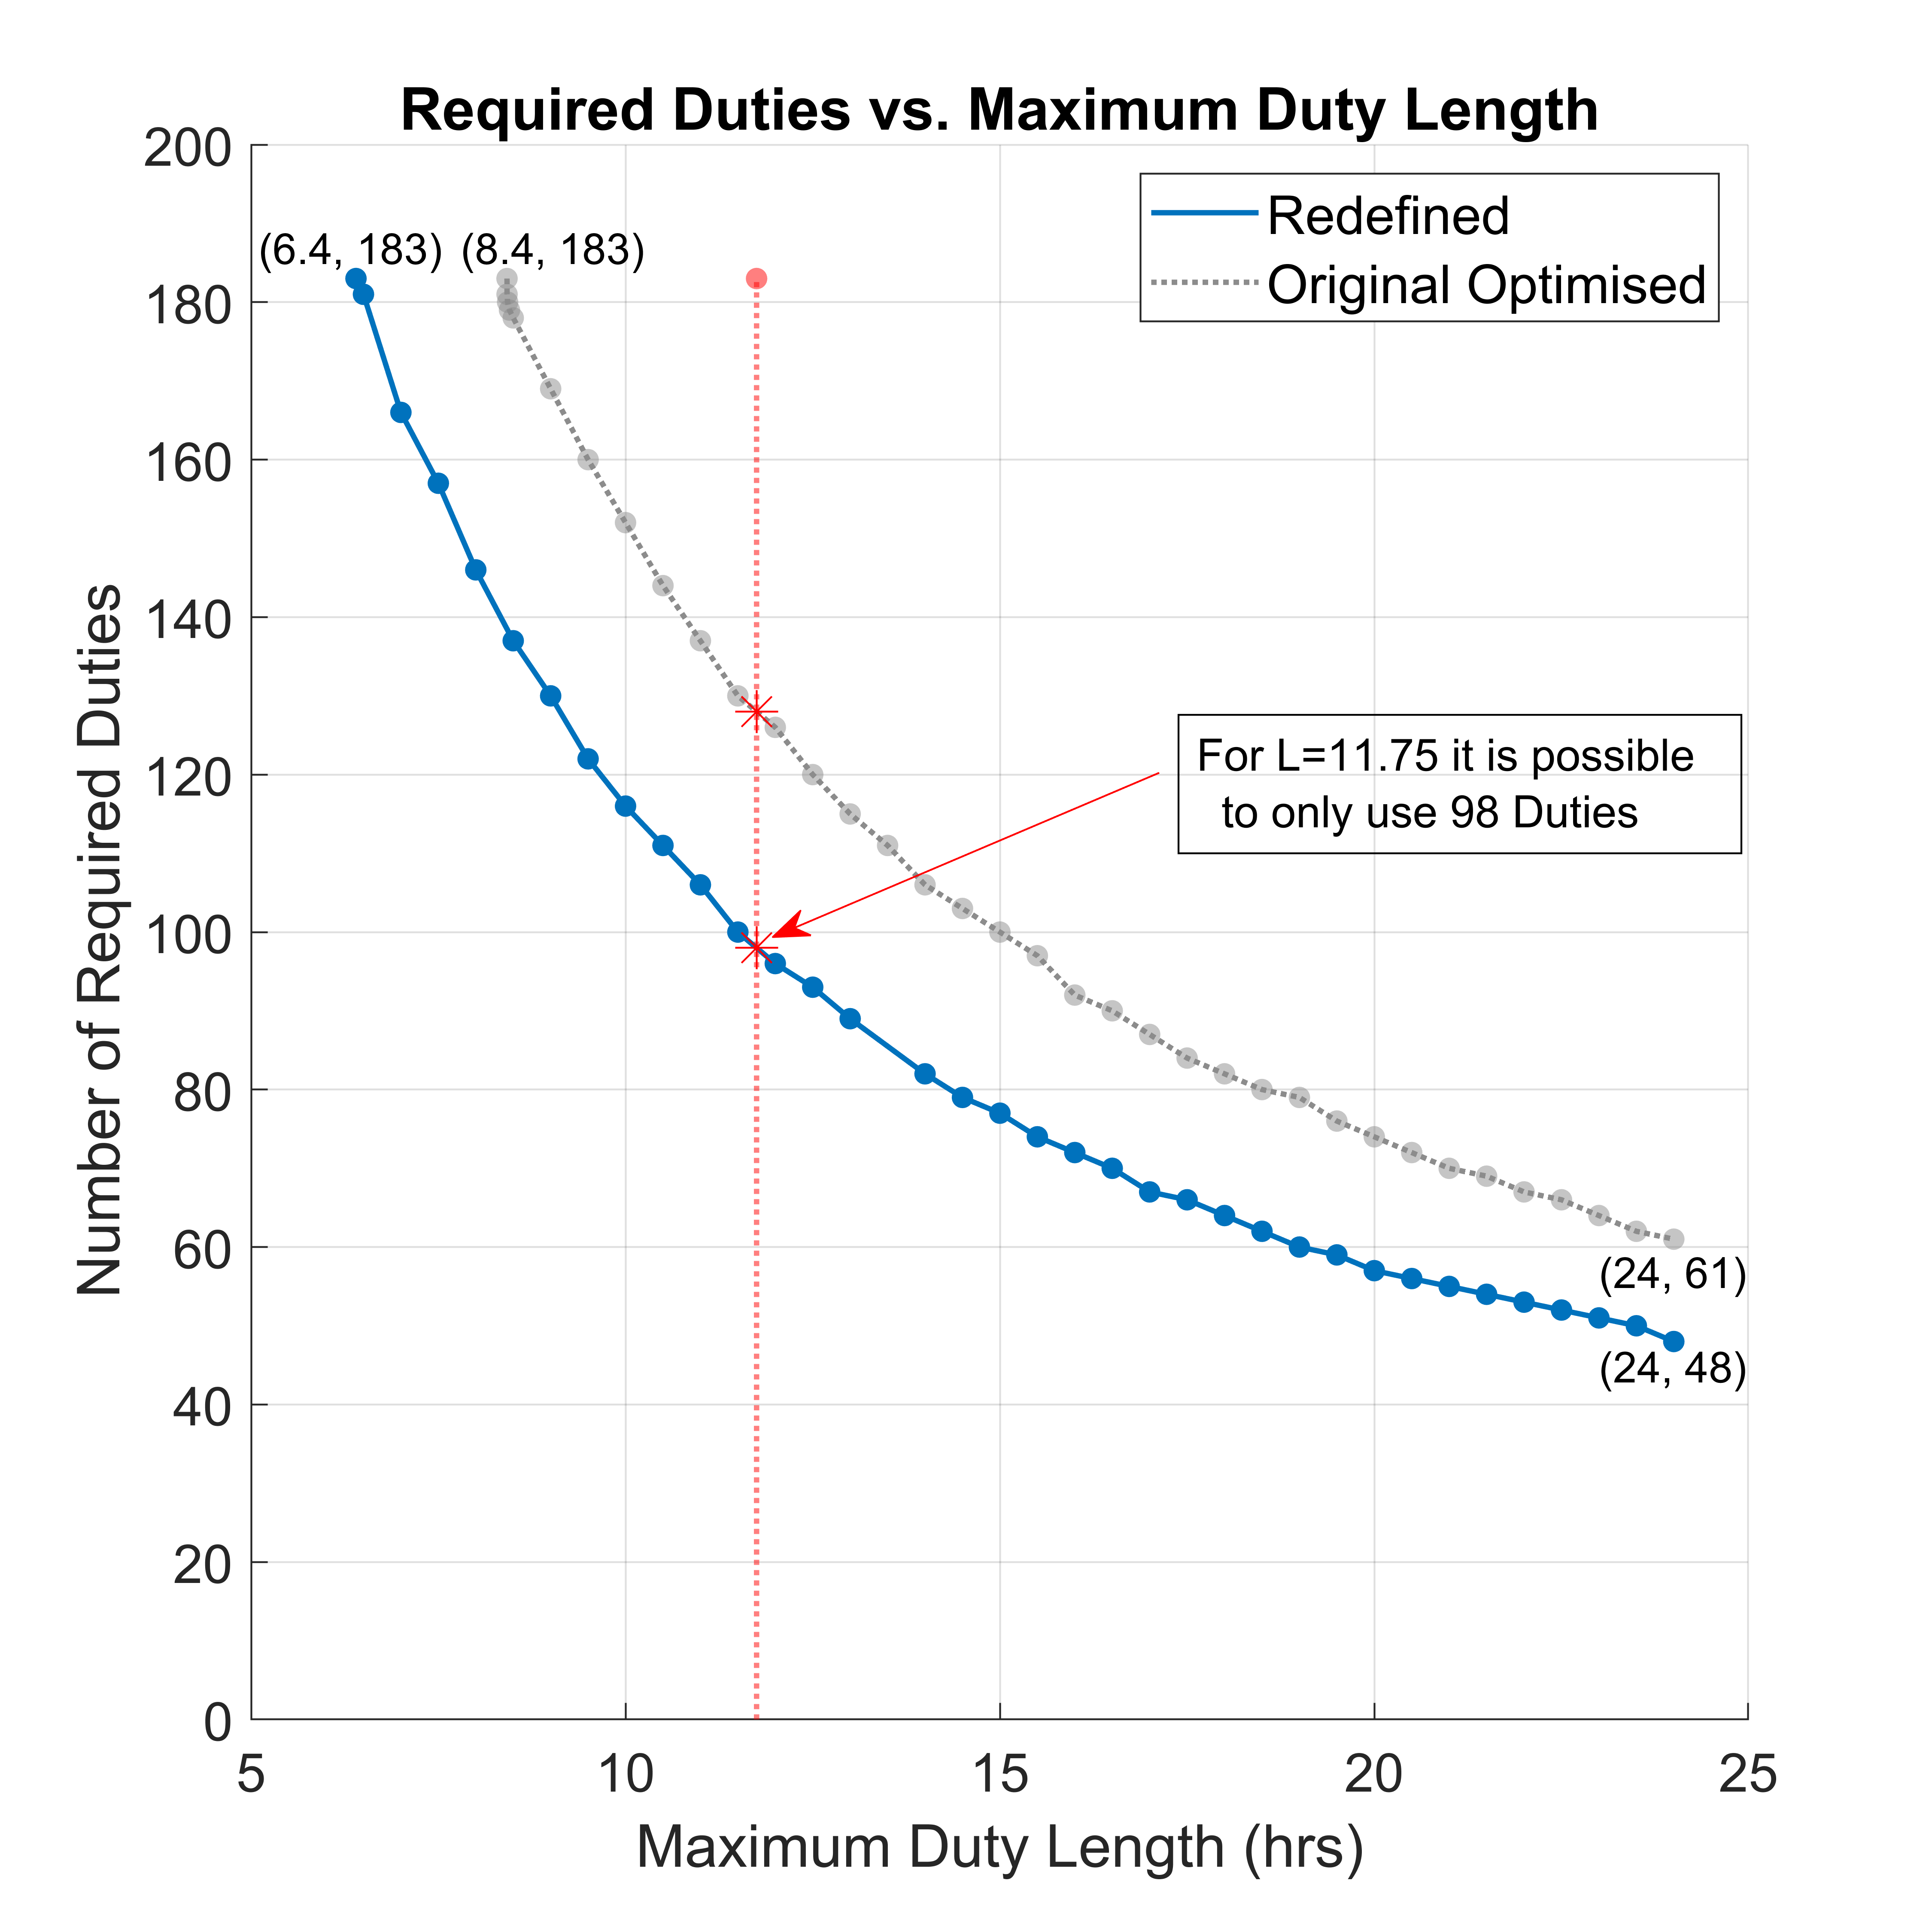
\includegraphics[width=0.46\linewidth]{[1] - chapter/Image Files/1-D2M2.png}
    \caption{Compares the number of duties required as a function of the Maximum Duty Length for the Redefined and Historical instances.}
    \label{fig:1-D2M2}
\end{figure}


%%%%%%%%%%%%%%%%%%%%%%%%%%%%%%%%%%%%%%%%%%%%%%%%%%%%%%%%%%%%%%%%%%%%%%%%%%%%%%% sub-SECTION %%%%%%%%%%%%%%%%%%%%%%%%%%%%%%%%%%%%%%%%%%%%%%%%%%%%%%%%%%%%%%%%%%%%%%%%%%%%%%


\subsection*{Evaluation - Optimising Redefined Instance}
We proceed to apply the Redefined instance, to model (\ref{equation: Minimise Duties}) in order to determine whether applying this more realistic instance will further improve the two objectives of our problem. For the historical instance, our optimisation was able to minimise the number of duties by around 30\% for an \textit{L} equal to Royal Mail's historical threshold. When applying the Redefined instance we expect an additional decrease in the number of required duties for the same \textit{L}. The expectation is founded in the fact that, in this new instance there is less overall schedulable time. Hence, that means that for the same maximum duty length, we can fit more blocks per duty which will directly result in less duties being used overall. 

\vspace{\baselineskip}
\noindent
Indeed, were able to carry out the same amount of block with \textbf{47\%} less duties, namely merely 96 duties as seen in Figure \ref{fig:1-D2M2}. This result justifies our quest for optimisation, since it identifies that Royal Mail's current practices are once again outside the \textit{efficient frontier} line. 

\vspace{\baselineskip}
\noindent
Observing the Figure \ref{fig:1-D2M2}, we can see that this additional reduction in required duties, is mostly due to the step change in \textit{idle time} that we are able to achieve from deleting the \textit{non-useful} activities within the blocks. However, as is shown in Section \ref{section: Redefined Dataset} the idle time that we gain is on average 1 hour and 44 minutes per duty. Moreover, we saw in Section \ref{section:Makespan Scheduling-content} that the average size of a block is on average 2 hours and 25 minutes for the Redefined instance. As a result of those two facts we can determine why the application of the model on the Redefined yields only an additional small improvement of 17\% in the number of duties deleted compared to the 30\% improvement obtained in the Historical instance. The explanation is found in the fact despite the increase in idle time there is still not enough space to re-allocate the deleted duties' blocks to other duties, since the average idle time gain (of 01:44) per duty, is significantly smaller than the average size of the block (02:25), hence there are generally not too many blocks that can be relocated to other duties so that we can delete their original duty.


\vspace{\baselineskip}
\noindent
Once again, if we attempt to determine the \textbf{theoretical optimal schedule} for the Redefined instance we would expect to obtain a schedule with maximum duty length (\textit{L}) of 6 hours and 06 minutes\footnote{Such that \textit{L} coincides with the Redefined schedule's average duty length seen in Section \ref{section: Redefined Dataset}}. Given that as we saw in Figure \ref{fig:1-D2M2} we can only go as low as an  $L=6.4 \text{ hours}$\footnote{Which amounts to 6 hours and 24 minutes.}  we can see there exist an optimality gap between the schedule with the ideal maximum duty length and the one we can practically obtain. This is once again due to the fact that atomic blocks have an arbitrary size and hence the solver more often than cannot find a duty length that fits all blocks exactly. 
%%%%%%%%%%%%%%%%%%%%%%%%%%%%%%%%%%%%%%%%%%%%%%%%%%%%%%%%%%%%%%%%%%%%%%%%%%%%%%% SECTION %%%%%%%%%%%%%%%%%%%%%%%%%%%%%%%%%%%%%%%%%%%%%%%%%%%%%%%%%%%%%%%%%%%%%%%%%%%%%%
\section{Maximising the Number of Completed Duties with Limited Driver Time}
\label{section: maximise blocks}
Having created the sensitivity analysis that identified the minimum number of required duties for each value of \textit{L} we proceeded to solve the directly symmetric problem. More specifically, in Figure \ref{fig:1-D1M1} of Section \ref{section:minimise duties} the left end of the curve informed us that the most tight feasible schedule we can possible create is one where the maximum duty length (\textit{L}) is equal to 8.417 hours. Being aware aware of that we would like to move towards infeasibility and discover the schedules that are to the left of that Pareto optimal schedule with $L=8.417 \text{ hours}$.

\vspace{\baselineskip}
\noindent
The reasoning behind conducting this experiment is to determine the effect the decrease of \textit{L} and the transition towards infeasibility will have on the processing capacity of the MC. More specifically, given that we are moving towards infeasibility, we are aware that we will no longer be able to create a feasible schedule, i.e. a schedule that manages to fit in all blocks, since we have determined that an $L=8.417 \text{ hours}$ is the least maximum duty length that can fit all the 183 blocks. Hence, further decreasing \textit{L} will certainly result in not enough schedulable time to fit all the blocks inside the schedule. 

\vspace{\baselineskip}
\noindent
The practical purpose of this experiment is to investigate the degree to which we see a degradation in the processing capacity of the MC as we decrease \textit{L}. In practice to perform this experiment we maximise the number of blocks that can be completed for each value of \textit{L}, by creating another sensitivity analysis. By decreasing $L$ we obviously will no longer be able to complete everything, so the question posed is what is the maximum amount of work (i.e. number of blocks) that we can manage to accomplish for each \textit{L}. 

%%%%%%%%%%%%%%%%%%%%%%%%%%%%%%%%%%%%%%%%%%%%%%%%%%%%%%%%%%%%%%%%%%%%%%%%%%%%%%% Maths %%%%%%%%%%%%%%%%%%%%%%%%%%%%%%%%%%%%%%%%%%%%%%%%%%%%%%%%%%%%%%%%%%%%%%%%%%%%%%

\vspace{\baselineskip}
\begin{equation}
\label{equation: M3}
\begin{aligned}
&\text{maximise}
& & \sum _{i=1}^m x_{i,j}  \\
& \text{subject to}
& &\sum _{i=1}^m x_{i,j} \leq 1 \;\;\; &\forall \; j \in B\\
& & &\sum _{j=1}^n x_{i,j}p_{j} \leq L \;\;\; &\forall \; i \in D\\
& & & y\geq 0  \\
& & & x_{i,j} \in  \{ 0,1 \} \;\;\; &\forall \; j \in B, \; i \in D\\
\end{aligned}
\end{equation}

\vspace{\baselineskip}
\noindent
The model maximises the number of blocks processed, for the given constraints. The first constraint applies the allowance of non-feasible schedules. It allows for a block to not be processed by a duty. The third constraint makes sure that the contents of a duty do not exceed the maximum duty length threshold $L$ as seen in the previous formulation. This maximum duty length is varied to then complete the sensitivity analysis. 

%%%%%%%%%%%%%%%%%%%%%%%%%%%%%%%%%%%%%%%%%%%%%%%%%%%%%%%%%%%%%%%%%%%%%%%%%%%%%%% Figure %%%%%%%%%%%%%%%%%%%%%%%%%%%%%%%%%%%%%%%%%%%%%%%%%%%%%%%%%%%%%%%%%%%%%%%%%%%%%%

\begin{figure}
    \centering
    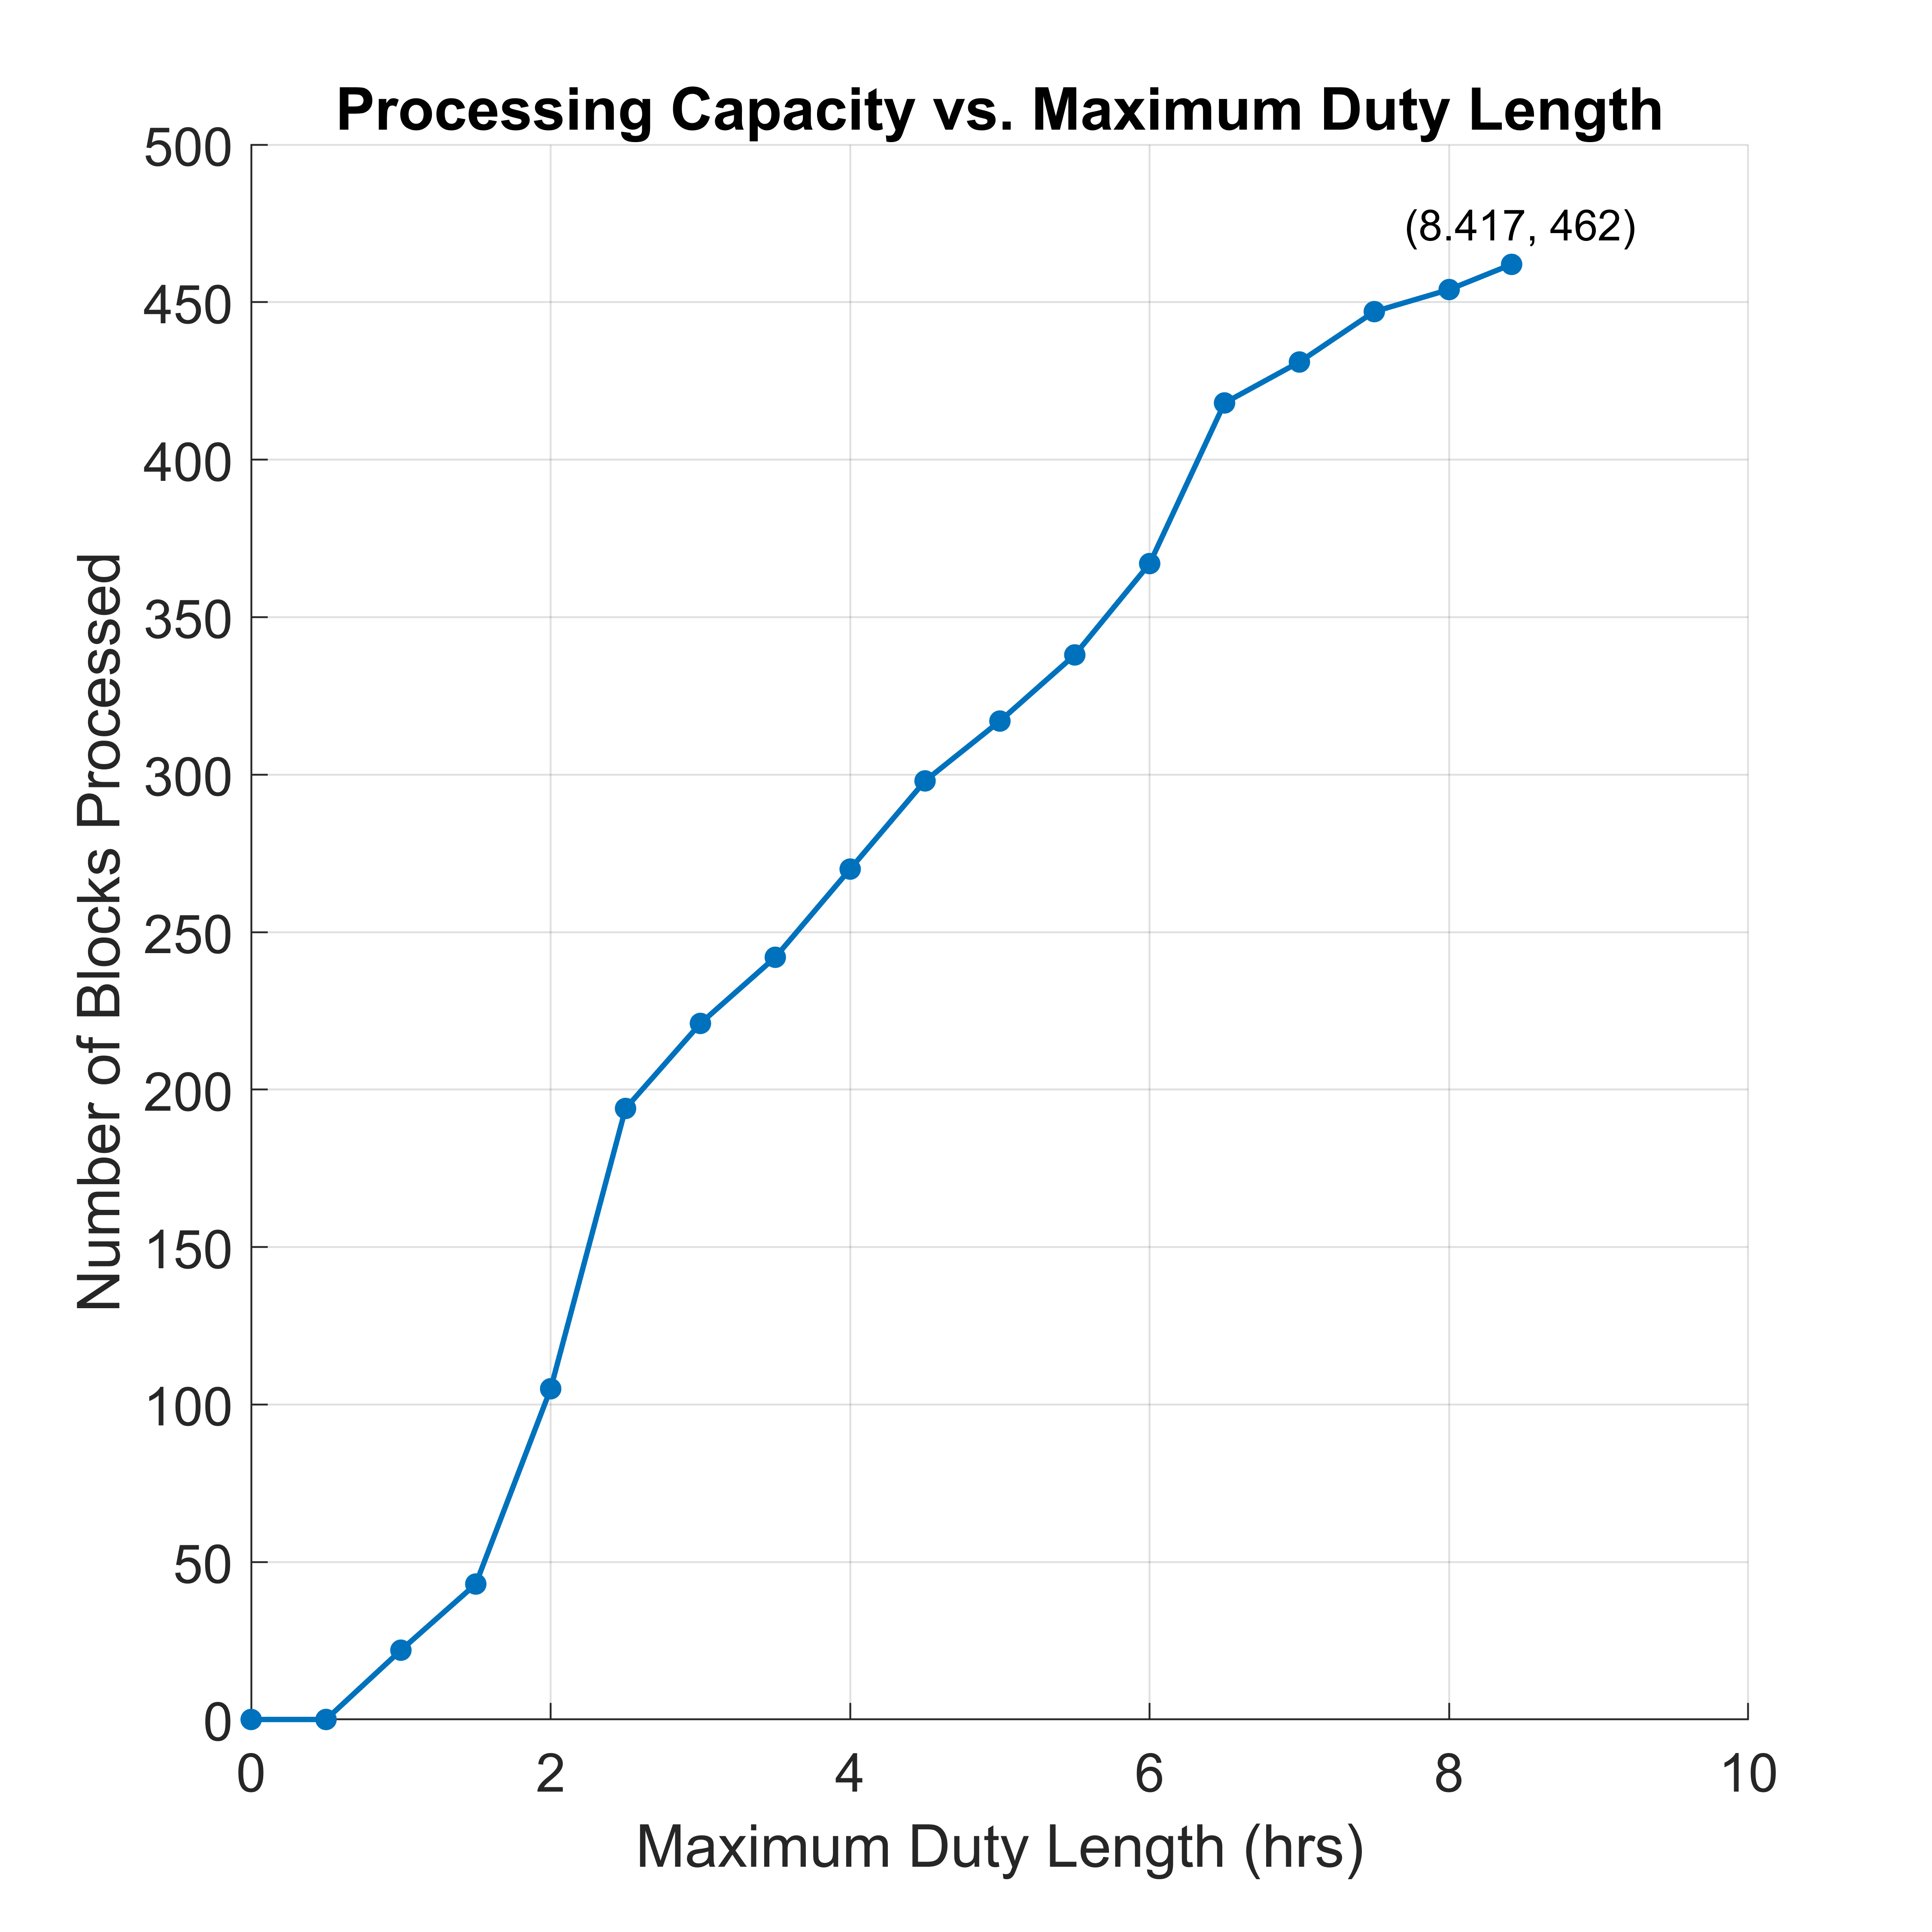
\includegraphics[width=0.46\linewidth]{[1] - chapter/Image Files/1-D1M3.png}
    \caption{Depicts the number of blocks that can be processed as a function of the Maximum Duty Length varied in 30 minute intervals, up to an \textit{upper threshold} that provides the first schedule that is feasible.}
    \label{fig:1-D1M3}
\end{figure}


%%%%%%%%%%%%%%%%%%%%%%%%%%%%%%%%%%%%%%%%%%%%%%%%%%%%%%%%%%%%%%%%%%%%%%%%%%%%%%% sub-SECTION %%%%%%%%%%%%%%%%%%%%%%%%%%%%%%%%%%%%%%%%%%%%%%%%%%%%%%%%%%%%%%%%%%%%%%%%%%%%%%

\subsection*{Evaluation}
Applying equation (\ref{equation: M3}) to the \textbf{historical} instance and by repeating this process in conjunction with the Pareto algorithm (\ref{alg: Pareto}) 18 times we receive the curve \ref{fig:1-D1M3} depicting the results of the sensitivity analysis. In the study of this problem we keep the amount of duties fixed to 183 available, and are only concerned with the effects on the processing capacity of the schedule (i.e. the amount of blocks that can fit in those duties).

\subsubsection*{Qualitative Results}
The trade-off curve shows the efficient frontier that we have created in its entirety. The frontier, shows us that as expected while we decrease the value of \textit{L} the schedules that we are able to create have an ever-decreasing processing capacity since as we can see they are able to process a continuously decreasing amount of blocks. The right end of the curve shows the only feasible schedule featured on this curve. That point with $L=8.417 \text{ hours}$ is the meeting point between the problem that we are currently solving and its symmetric that was studied in Section \ref{section:minimise duties}. The symmetry of the two problems is confirmed through this function since the schedule rightmost schedule of Figure \ref{fig:1-D1M3} coincides with the leftmost schedule of Figure \ref{fig:1-D1M2} since they both refer to schedules with 183 duties, 462 blocks processed and an $L=8.417 \text{ hours}$.

\subsubsection*{Quantitative Results}
Another interesting finding concerns the relationship between the degradation of the processing capacity as a function of \textit{L}. As we can see in Figure \ref{fig:1-D1M3} if we reduce the duty length by 2 hours, (\textbf{25\% reduction}), the decrease in duties that can be performed is only of the order of magnitude of \textbf{10\%}. This finding is in the direction of obtaining the trade-off relationship between finding the maximum duty length and the effect it has on the processing capacity of the MC. A practical understanding provided by this finding is that if we decrease \textit{L} by this 2 hour interval i.e. down to around 6 and a half hours, we will not have a proportional decrease in the processing capacity. From the perspective of Royal Mail, this insight could mean that we could allow a small portion of people to work part-time if they so wish. This insight is explained by the fact that this group of part-time employees could carry out that \textbf{10\%} of blocks that are left unscheduled. Moreover, since they would only work part-time they would work considerably less hours, hence allowing for the decrease seen in \textit{L} of the order of textbf{25\%}. These insights are not concrete proof that this would work for Royal Mail, but they show that significantly reducing drivers' work time results in a not so significant reduction in the number of blocks that can be processed.

\subsection*{Evaluation - Optimising Redefined Instance}

%%%%%%%%%%%%%%%%%%%%%%%%%%%%%%%%%%%%%%%%%%%%%%%%%%%%%%%%%%%%%%%%%%%%%%%%%%%%%%% Figure %%%%%%%%%%%%%%%%%%%%%%%%%%%%%%%%%%%%%%%%%%%%%%%%%%%%%%%%%%%%%%%%%%%%%%%%%%%%%%

\begin{figure}%
    \centering
    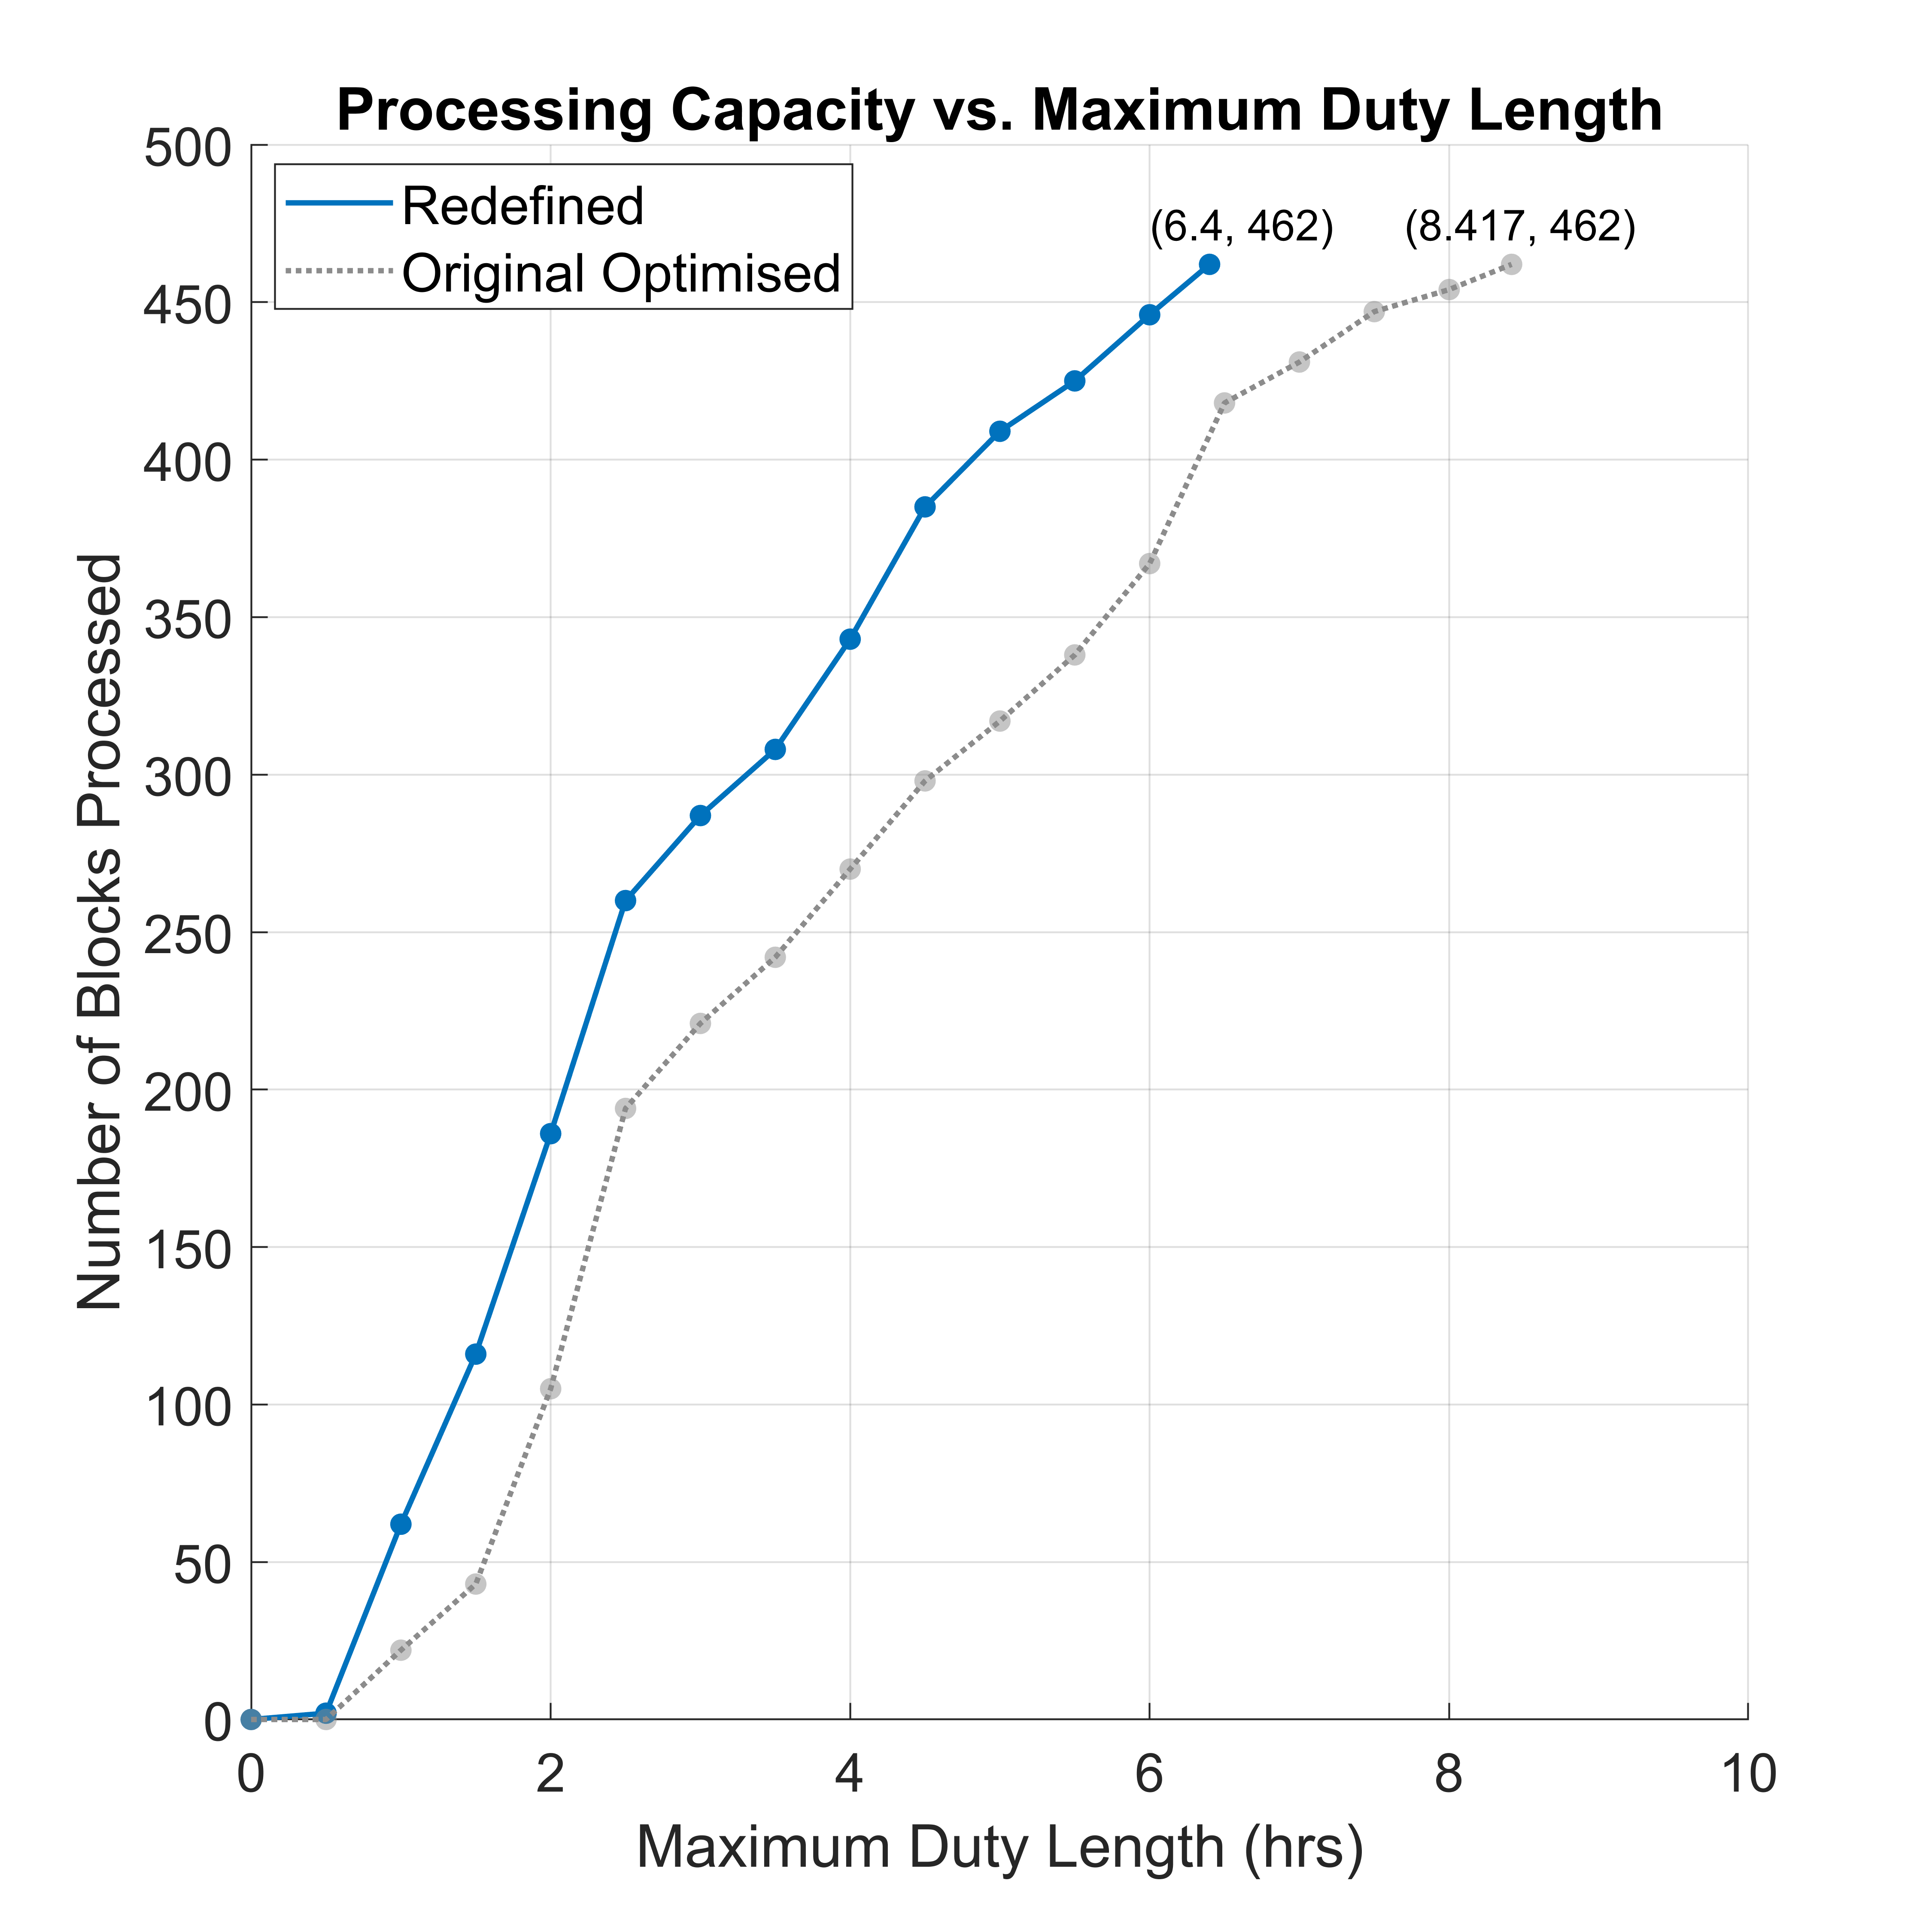
\includegraphics[width=0.46\linewidth]{[1] - chapter/Image Files/1-D2M3.png}
    \caption{Compares the number of blocks that can be processed as a function of the Maximum Duty Length for the Redefined and Historical instances.}
    \label{fig:1-D2M3}
\end{figure}

\vspace{\baselineskip}
\noindent
In a similar fashion to the case of the results from the Redefined instances in Section \ref{section:minimise duties}, the application of the Redefined instances provides marginally better results. In more detail, as seen in Figure \ref{fig:1-D2M3}, the processing capacity of the schedules generated based on the Redefined instances is hindered ever so slightly less, in comparison to the Historical instance's. That is an expected phenomenon, since as we mentioned before the blocks of the Redefined instances, contain naturally smaller blocks, since they do not consider the redundant activities. As a result, more of them can generally fit in the same 183 duties, which explains the smaller degradation in the processing capacity for the same level of \textit{L} compared to the Historical instance's schedules. 
%%%%%%%%%%%%%%%%%%%%%%%%%%%%%%%%%%%%%%%%%%%%%%%%%%%%%%%%%%%%%%%%%%%%%%%%%%%%%%% SECTION %%%%%%%%%%%%%%%%%%%%%%%%%%%%%%%%%%%%%%%%%%%%%%%%%%%%%%%%%%%%%%%%%%%%%%%%%%%%%%

\section{Load Balancing with Pre-emptions}
\label{section: Pre-emptive}
The final experiment run in this chapter involves the further investigation of the \textbf{theoretical optimal schedule} discussed in the final parts of the evaluations of the prior sections. In all three prior sections, we saw that there exists an absolute theoretical limit that would give us the corresponding \textbf{theoretical optimal schedule} with respect to the makespan objective. However, we also saw that the most optimal schedules that our solver was able to come up with would always have a certain optimality gap to that theoretical schedule. That theoretical schedule has been obtained through theoretically hypothesising that we can split the total schedulable labor hours equally in duties of equal length. Unlike, the other schedules discussed in this chapter it has not been obtain as an output from our solver. The purpose of exploring this topic is to investigate how close we can get to that theoretical limit with a schedule generated by our solver if we relax some of the design principles of our makespan formulation. 

\vspace{\baselineskip}
\noindent
It is normal to expect that completely achieving the theoretical limit is not a possibility. That is because as explained in the previous sections to obtain that theoretically optimal schedule we would have to completely disregard the structure of our components. Namely, we would have to discretise our activities and blocks with a very high frequency, effectively rendering them a collection of time instants that can exactly fit in duties of any length. However, that experiment is of little utility to us. In investigating how close we can get to approaching the theoretical limit, we choose to only breakdown the size of the blocks, but maintain the structure and processing times of the activities intact. Hence, we still expect not to be able to completely approach the theoretical limit, because cases where activities lengths' do not exactly fit in duties are expected to occur.  


\vspace{\baselineskip}
\noindent
To develop a schedule that approaches the theoretical limit we ran the MIP seen in Section \ref{section:Makespan Scheduling-content}, but by allowing the model to act \textbf{preemptively}. Non-pre-emptive formulations were used in all previous three models. By disregarding this design parameter we grant the model complete freedom in terms of the policy with which it can process each block. Effectively, we provide it with an additional degree of freedom that allows it to switch between blocks while processing one already. Effectively, it is allowed to process activities from different blocks even after having begun the processing of an activity from a different block. 

\vspace{\baselineskip}
\noindent
In practice, we carry this out by supplying instances of $I = \langle{m},\langle{B},A\rangle{}$ of the problem in an environment of $D=\{1,...,m\}$ parallel duties. However, in addition to a set of blocks we provide a set of activities $A =\{1,...,n\}$. The Historical instance utilised contained 3,285 activities that were allocated once again among a set of 183 duties. 

\vspace{\baselineskip}
\noindent
Through supplying activities as the component to be scheduled, the model is now \textbf{pre-emptive} with respect to blocks, since the solver is allowed to move activities around within each duty hence, breaking the original structure of the blocks. Consequently, we have allowed the model to switch between blocks by allowing it to start processing an activity from one block and then switch to processing an activity from a different block. The activities $j \in A$ all have their processing time $p_{j}$ as before. 

\vspace{\baselineskip}
\noindent
The \textit{MILP} is marginally changed. The biggest change is seen in the constraint: $\sum _{i=1}^m x_{i,j} = 1$ which is converted to $\sum _{i=1}^m x_{i,j} = p_j$ \cite{DUMMY:2}. Moreover $x_{i,j}$ are no longer binary variables. Variables $x_{i,j}$ now represent the time each block spends on each machine compared to whether machine \textit{i} executes job \textit{j} as before.

\vspace{\baselineskip}
\noindent
As a result formulation (\ref{equation: Makespan Scheduling}) from Section \ref{section:Makespan Scheduling-content} becomes:

%%%%%%%%%%%%%%%%%%%%%%%%%%%%%%%%%%%%%%%%%%%%%%%%%%%%%%%%%%%%%%%%%%%%%%%%%%%%%%% Maths %%%%%%%%%%%%%%%%%%%%%%%%%%%%%%%%%%%%%%%%%%%%%%%%%%%%%%%%%%%%%%%%%%%%%%%%%%%%%%

\vspace{\baselineskip}
\begin{equation}
\label{equation: Makespan preemptive}
\begin{aligned}
&\text{minimise}
%& & y_{i}  \\ %\todo{why y and and not yi}
& & y  \\ 
& \text{subject to}
% & & y_{i} = \sum _{j=1}^n x_{i,j}p_{j}  \;\;\; &\forall \; i \in D\tag{1}\\   
& & y\geq \sum _{j=1}^n x_{i,j}  \;\;\; &\forall \; i \in D\\   
& & &\sum _{i=1}^m x_{i,j} = p_j \;\;\; &\forall \; j \in B\\
& & &y \geq \sum _{i=1}^m x_{i,j}  \;\;\; &\forall \; j \in B\\
% & & &\sum _{j=1}^n x_{i,j}p_{j} \leq f_{i}-s_{i} \;\;\; &\forall \; i \in D\\ %{\color{red} we deleted the constraint that involves the length of duty being less than end-start.}
& & & y,x_{i,j}\geq 0  \\
\end{aligned}
\end{equation}

\vspace{\baselineskip}
\noindent
The problems objective is once again to minimise the \textbf{makespan} while obtaining a feasible schedule. The first constraint assigns $y$ its definition of the \textbf{makespan}, since the makespan must be greater or equal to the completion time of the longest lasting machine. With the second constraint we ensure that each job is performed to completion on the various machines that process it. The final constraint ensures that no block is processed for more total time than the makespan itself.

%%%%%%%%%%%%%%%%%%%%%%%%%%%%%%%%%%%%%%%%%%%%%%%%%%%%%%%%%%%%%%%%%%%%%%%%%%%%%%% sub-SECTION %%%%%%%%%%%%%%%%%%%%%%%%%%%%%%%%%%%%%%%%%%%%%%%%%%%%%%%%%%%%%%%%%%%%%%%%%%%%%%

\subsection*{Evaluation}
To investigate how close we can approach to the theoretical limit of the maximum duty length, we attempt through this experiment to establish a practical lower-bound solution. As mentioned in the beginning of this section, we do not expect to achieve the \texttt{absolute theoretical limit}. But by investigating the effects a preemptive model would have on our results, we can obtain a realisable best possible solution that we can hope to achieve. The \texttt{absolute theoretical limit} is that of a maximum duty length equal to the average duty length of the instance, which in the case of the Historical instance is equal to 7 hours and 50 minutes.

\vspace{\baselineskip}
\noindent
The results of the preemptive model hints to a lower-bound for the maximum duty length of 8 hours and 5 minutes. Compared to the makespan of 8 hours and 25 minutes this is a significant improvement in the maximum duty length. In fact this is a \textbf{7\%} improvement in the optimality gap with the \texttt{absolute theoretical limit}. 

%%%%%%%%%%%%%%%%%%%%%%%%%%%%%%%%%%%%%%%%%%%%%%%%%%%%%%%%%%%%%%%%%%%%%%%%%%%%%%% sub-SECTION %%%%%%%%%%%%%%%%%%%%%%%%%%%%%%%%%%%%%%%%%%%%%%%%%%%%%%%%%%%%%%%%%%%%%%%%%%%%%%

\subsection*{Evaluation - Optimising Redefined Instances}
We repeat the process outlined above to calculate the effect of pre-emption on the Redefined instance. We ran the MILP (\ref{equation: Makespan preemptive}) but with an instance containing 2,850 activities that were once again allocated among a set of 183 duties. The \texttt{absolute theoretical limit} in this case would be to obtain a schedule where \textit{L} would be equal to the average duty length of the instance (i.e. 06:06). 

\vspace{\baselineskip}
\noindent
Upon running the pre-emptive model on the instance we obtain a practical lower-bound of 6 hours and 32 minutes. Similar to the prior case of the Historical instance this is a significant improvement over the previously obtained makespan of 7 hours and 27 minutes. In quantitative terms this is a bigger improvement compared to the Historical instance's case, of magnitude \textbf{23\%}.